\documentclass [11pt,twoside]{article}
\usepackage[utf8]{inputenc}
\usepackage[T1]{fontenc}

%Page margins, header and footer positions
\usepackage{geometry}
 \geometry{
 a4paper,
 total={210mm,297mm},
 left=25mm,
 right=25mm,
 top=30mm,
 bottom=25mm,
 headsep=7mm}

\interfootnotelinepenalty=10000

%To display filling dots in the TOC for all entries
\usepackage[titles]{tocloft}
\renewcommand{\cftsecleader}{\cftdotfill{\cftdotsep}}

%Define new header and footer style
\usepackage{fancyhdr}

\pagestyle{fancy}
\fancyhf{}
\lhead{\color{Gray}{\small{S\&C project by Edoardo S. Gribaldo and Federico Rosa}}}
\lfoot{\textcolor{Gray}{\small{Copyright © 2025, Edoardo S. Gribaldo and Federico Rosa – All rights reserved}}}
\rfoot{\textcolor{Gray}{\thepage}}
\renewcommand{\headrulewidth}{0pt}

%PACKAGES
\usepackage{wasysym}
\usepackage{pifont}

\newcommand{\supported}{\ding{52}\xspace}
\newcommand{\unsupported}{\ding{55}\xspace}
\newcommand{\partsupported}{\textcolor{black!40}{\ding{52}}\xspace}
\newcommand{\lowsupported}{\textcolor{black!20}{\ding{52}}\xspace}
\newcommand{\unknowsupported}{\textbf{?}\xspace}

%Font: Times
\usepackage{times}
%Change monospaced font
\renewcommand{\ttdefault}{lmtt}

%tables
\usepackage{tabu}
\usepackage{tabularx}
\usepackage{ltablex}
\usepackage{longtable}
\usepackage{float} % To allow the use of H modifier in long tables

%landscape mode
\usepackage{pdflscape}
\usepackage{rotating}
\usepackage{caption}

%make landscape mode be sensitive to even and odd pages
%start
\def\myrotate{\ifodd\c@page\else-\fi 90}
\makeatletter
\global\let\orig@begin@landscape=\landscape%
\global\let\orig@end@landscape=\endlandscape%
\gdef\@true{1}
\gdef\@false{0}
\gdef\landscape{%
    \global\let\within@landscape=\@true%
    \orig@begin@landscape%
}%
\gdef\endlandscape{%
    \orig@end@landscape%
    \global\let\within@landscape=\@false%
}%
\@ifpackageloaded{pdflscape}{%
    \gdef\pdf@landscape@rotate{\PLS@Rotate}%
}{
    \gdef\pdf@landscape@rotate#1{}%
}
\let\latex@outputpage\@outputpage
\def\@outputpage{
    \ifx\within@landscape\@true%
        \if@twoside%
            \ifodd\c@page%
                \gdef\LS@rot{\setbox\@outputbox\vbox{%
                    \pdf@landscape@rotate{-90}%
                    \hbox{\rotatebox{90}{\hbox{\rotatebox{180}{\box\@outputbox}}}}}%
                }%
            \else%
                \gdef\LS@rot{\setbox\@outputbox\vbox{%
                    \pdf@landscape@rotate{+90}%
                    \hbox{\rotatebox{90}{\hbox{\rotatebox{0}{\box\@outputbox}}}}}%
                }%
            \fi%
        \else%
            \gdef\LS@rot{\setbox\@outputbox\vbox{%
                \pdf@landscape@rotate{+90}%
                \hbox{\rotatebox{90}{\hbox{\rotatebox{0}{\box\@outputbox}}}}}%
            }%
        \fi%
    \fi%
    \latex@outputpage%
}
\makeatother
%end

%graphics
\usepackage{graphicx}
\usepackage[dvipsnames, table]{xcolor}
%If you upload images from PC, you need to insert code for the path here (different for Windows and Unix OS)

%References
%\usepackage{xpatch}
%\usepackage[backend=biber, style=numeric, citestyle=numeric, sorting=none]{biblatex}
%\addbibresource{main.bib}

%Other
\usepackage{ifthen}
\usepackage{xspace}
\usepackage{enumitem}
\usepackage{amssymb}
\usepackage[pdftex, colorlinks]{hyperref}
\newcommand{\comment}[1]{{\color{Red}$\blacktriangleright$ Comment: #1 $\blacktriangleleft$}}


% Some utilities\ldots
\usepackage{soul}
\usepackage{tikz}

\usetikzlibrary{calc}
\usetikzlibrary{decorations.pathmorphing}


\makeatletter

\newcommand{\defhighlighter}[3][]{%
  \tikzset{every highlighter/.style={color=#2, fill opacity=#3, #1}}%
}

\defhighlighter{yellow}{.5}

\newcommand{\highlight@DoHighlight}{
  \fill [ decoration = {random steps, amplitude=1pt, segment length=15pt}
        , outer sep = -15pt, inner sep = 0pt, decorate
       , every highlighter, this highlighter ]
        ($(begin highlight)+(0,8pt)$) rectangle ($(end highlight)+(0,-3pt)$) ;
}

\newcommand{\highlight@BeginHighlight}{
  \coordinate (begin highlight) at (0,0) ;
}

\newcommand{\highlight@EndHighlight}{
  \coordinate (end highlight) at (0,0) ;
}

\newdimen\highlight@previous
\newdimen\highlight@current

\DeclareRobustCommand*\highlight[1][]{%
  \tikzset{this highlighter/.style={#1}}%
  \SOUL@setup
  %
  \def\SOUL@preamble{%
    \begin{tikzpicture}[overlay, remember picture]
      \highlight@BeginHighlight
      \highlight@EndHighlight
    \end{tikzpicture}%
  }%
  %
  \def\SOUL@postamble{%
    \begin{tikzpicture}[overlay, remember picture]
      \highlight@EndHighlight
      \highlight@DoHighlight
    \end{tikzpicture}%
  }%
  %
  \def\SOUL@everyhyphen{%
    \discretionary{%
      \SOUL@setkern\SOUL@hyphkern
      \SOUL@sethyphenchar
      \tikz[overlay, remember picture] \highlight@EndHighlight ;%
    }{%
    }{%
      \SOUL@setkern\SOUL@charkern
    }%
  }%
  %
  \def\SOUL@everyexhyphen##1{%
    \SOUL@setkern\SOUL@hyphkern
    \hbox{##1}%
    \discretionary{%
      \tikz[overlay, remember picture] \highlight@EndHighlight ;%
    }{%
    }{%
      \SOUL@setkern\SOUL@charkern
    }%
  }%
  %
  \def\SOUL@everysyllable{%
    \begin{tikzpicture}[overlay, remember picture]
      \path let \p0 = (begin highlight), \p1 = (0,0) in \pgfextra
        \global\highlight@previous=\y0
        \global\highlight@current =\y1
      \endpgfextra (0,0) ;
      \ifdim\highlight@current < \highlight@previous
        \highlight@DoHighlight
        \highlight@BeginHighlight
      \fi
    \end{tikzpicture}%
    \the\SOUL@syllable
    \tikz[overlay, remember picture] \highlight@EndHighlight ;%
  }%
  \SOUL@
}

\makeatother

% Common abbrev. are set as commands to ensure proper spacing after the dot
\RequirePackage{xspace}
\newcommand{\ie}{i.e.\@\xspace}
\newcommand{\aka}{a.k.a.\@\xspace}
\newcommand{\Ie}{I.e.\@\xspace}
\newcommand{\cf}{cf.\@\xspace}
\newcommand{\Cf}{Cf.\@\xspace}
\newcommand{\eg}{e.g.\@\xspace}
\newcommand{\Eg}{E.g.\@\xspace}
\newcommand{\etal}{et al.\@\xspace}
\newcommand{\etc}{etc.\@\xspace}
\newcommand{\wrt}{w.r.t.\@\xspace}
\newcommand{\Wrt}{W.r.t.\@\xspace}



\date{}


\begin{document}

%TITLE PAGE

\begin{titlepage}


%LOGO

{\begin{table}[t!]
\centering
\begin{tabu} to \textwidth { X[1.3,r,p] X[1.7,l,p] }
\textcolor{Blue}
{\textbf{\small{Travlendar+ project YOUR NAMES}}} & 
\includegraphics[scale=0.5]{Images/PolimiLogo}
\end{tabu}
\end{table}}~\\ [7cm]

%TITLE 

\begin{flushleft}

%Replace the text string with your title
{\textcolor{Blue}{\textbf{\Huge{Requirement Analysis and Specification
        Document}}}} \\ [1cm]

\end{flushleft}

\end{titlepage}

%Define deliverable specific info
%Replace cell contents where needed
\begin{table}[h!]
\begin{tabu} to \textwidth { X[0.3,r,p] X[0.7,l,p] }
\hline

\textbf{Deliverable:} & RASD\\
\textbf{Title:} & Requirement Analysis and Verification Document \\
\textbf{Authors:} & YOUR NAMES \\
\textbf{Version:} & 1.0 \\ 
\textbf{Date:} & 31-January-2016 \\
\textbf{Download page:} & LINK TO YOUR REPOSITORY \\
\textbf{Copyright:} & Copyright © 2017, YOUR NAMES – All rights reserved \\
\hline
\end{tabu}
\end{table}




\setcounter{page}{2}


%------------------------------------------------------------------------------------------------------------------------------------------------
\newpage
\addcontentsline{toc}{section}{Table of Contents}
\tableofcontents
\newpage
\addcontentsline{toc}{section}{List of Figures}
\listoffigures
\addcontentsline{toc}{section}{List of Tables}
\listoftables

%------------------------------------------------------------------------------------------------------------------------------------------------
\clearpage
{\color{Blue}{\section{Introduction}}}
\label{sect:introduction}
%This document has been prepared to help you approaching Latex as a formatting tool for your Travlendar+ deliverables. This document suggests you a possible style and format for your deliverables and contains information about basic formatting commands in Latex. A good guide to Latex is available here \href{https://tobi.oetiker.ch/lshort/lshort.pdf}{https://tobi.oetiker.ch/lshort/lshort.pdf}, but you can find many other good references on the web. 

%Writing in Latex means writing textual files having a \texttt{.tex} extension and exploiting the Latex markup commands for formatting purposes. Your files then need to be compiled using the Latex compiler. Similarly to programming languages, you can find many editors that help you writing and compiling your latex code. Here \href{https://beebom.com/best-latex-editors/}{https://beebom.com/best-latex-editors/} you have a short oviewview of some of them. Feel free to choose the one you like.  

%Include a subsection for each of the following items\footnote{By the way, what follows is the structure of an itemized list in Latex.}:

% -----------------------------------------------------

\subsection{Purpose}
In today's job market, when looking for a job, having a previous work experience has become an important criteria of evaluation, therefore more and more students try to find an internship. On the other side, many companies are willing to invest into young talents in order to build a skilled workforce that can help them to drive innovation and foster and secure a competitive edge in the future. \\
Student\&Companies is a platform that offers to students the possibility to look up for internships and to companies the possibility of advertising. The matchmaking process of student and companies is enabled through a (proprietary) recommendation algorithm, that creates the most suited matches, through the collection of statistics and feedback. \\
Moreover Students\&Companies allows for the management of the selection process and the monitoring of the execution of the internships. The goal is to provide a platform for both students and companies to make the process of finding, offering and tracking internships easier and more efficient for both parties.

% ----

\subsubsection{Goals}
\begin{enumerate}[label={[G\arabic*]}]
    \item \textbf{Internship Lookup for Students}: 
    Help students in their search for an internship by connecting their profiles with well suited companies internship offers.
    \item \textbf{Internship Advertisement for Companies}: Enable companies to advertise their internships to students and inform them about availability of eligible candidates.
    \item \textbf{Selection Process Management}: Support the interaction and selection by providing a platform to companies to set up and conduct interviews, gather structured information about students and finalize the selections.
    \item \textbf{Data Collection for Recommendation System}: Collect statistics in order to allow the efficiency of the matchmaking process of the recommendation system 
    \item \textbf{Enhance Communication}: Enhance communication between students and companies, through a shared space where they can exchange information, raise problems and collect complaints about the internships
\end{enumerate}

% -----------------------------------------------------

\subsection{Scope}
The platform S\&C has two major stakeholders: students and companies. On one hand, students upload their CV and indicate their skills and domain of interest on the platform. Then they can proactively look out for internships or they can get suggestions from the platform, when new positions become available. On the other hand, companies can open internship positions, with the related domain and required skills, advertise those positions but also get notified when profiles of students, aligned with the requirements of one of their open positions, appear on the platform.
Once both parties express interest on the platform, a contact between the two is established. Then the management of the set up and the conduct of interview starts. When a candidate is selected, the platform tracks the conduction of the internship through feedback, complaints and exchange of information by both parties. Indeed a specific space of the website is devoted to communication between a student and company that have started an internship process together. The system run analytics on statistics collected by the platform itself on both students and companies to guarantee the best match possible between the two.

% ----

\subsubsection{World phenomena}
\begin{enumerate}[label={[WP\arabic*]}]
\item {Companies need interns for a position}
\item {Students write their own CVs}
\item {Students acquire new skills }
\item {Companies and students carry out internships on which they agreed upon}
\end{enumerate}

% ----

\subsubsection{Shared phenomena}
\begin{itemize}
    \item World controlled
    \begin{enumerate}[label={[SPWC\arabic*]}]
    
    \item {Companies create an internship position}
    \item {Companies carry out the selection process}
    \item {Companies select one student among the candidates}
    \item {Companies write complaints}
    \item {Companies communicate problems}
    \item {Students fill their profile with their personal information}
    \item {Students look out for an internship}
    \item {Students undertake assessments to test their skills on the platform}
    \item {Students write complaints}
    \item {Students communicate problems}
    
    
    \end{enumerate}
    \item Machine controlled
    \begin{enumerate}[label={[SPMC\arabic*]}]
    \item {The system notifies students of a newly available internship}
    \item {The system notifies the company of a newly available student that fits an internship role}
    \item {Contact between a student and a company is established} % I'm not sure it's Machine controlled
    \item {Companies provide feedback} % prompted by the system
    \item {Students provide feedback} % prompted by the system
    
    \end{enumerate}

\end{itemize}

% -----------------------------------------------------

\subsection{Definitions, Acronyms, Abbreviations}

\subsubsection{Definitions}
\begin{itemize}
    \item 
\end{itemize}

% ----

\subsubsection{Acronyms}
\begin{itemize}
    \item {S\&C: Students \& Companies}
    \item {UI: User Interface}
    \item {UML: Unified Modeling Language}
    \item {RASD: Requirement Analysis and Specification Document}
    \item {DD: Design Document}
\end{itemize}

% ----

\subsubsection{Abbreviations}
\begin{itemize}
    \item {G*: Goal}
    \item {WP*: World Phenomena}
    \item {SPWC*: Shared Phenomena World Controlled}
    \item {SPMC*: Shared Phenomena Machine Controlled}
    \item {FR*: Functional Requirement}
    \item {UC*: Use Case}
\end{itemize}

% -----------------------------------------------------

\subsection{Revision History}

% -----------------------------------------------------

\subsection{Reference Documents}
This document is based on the following reference documents:
\begin{itemize}
\item {The document of the 2024/2025 assignment for RASD and DD }
\item {The slides of the course found on WeBeep}
\end{itemize}

% -----------------------------------------------------

\subsection{Document Structure}
\begin{enumerate}
\item\textbf{Introduction}\\
The introduction identifies the purpose and the scope of the project, defines the goals, lists the related world and shared phenomena, explains acronyms, abbreviations that will be used in the document, specifies the version of the document and the reference document on which the current version it is based.
\item\textbf{Overall Description}\\
The overall description points out and explains the various scenarios, including class diagrams for the most difficult ones. It also includes product functions, user characteristics plus assumptions for the specific domain of the application, dependencies of the applications and constraints.
\item\textbf{Specific Requirements}\\
The specific requirements section defines the different interface and most importantly outlines all the functional requirements, alongside with all the possible use cases.
\item\textbf{Formal Analysis} \\
The part about formal analysis uses Alloy to formally verify the most difficult parts of the project
\item\textbf{Effort Spent}\\
The effort spent is described by a simple table
\item\textbf{References}\\
It has pointers to all the resources used or cited in this project
\end{enumerate}



%what you write here is a comment that is not shown in the final text

%------------------------------------------------------------------------------------------------------------------------------------------------
\clearpage
{\color{Blue}{\section{Overall Description}}}
\label{sect:overview}
%Here you can see how to include an image in your document.
%
%\begin{sidewaysfigure}
%\centering
%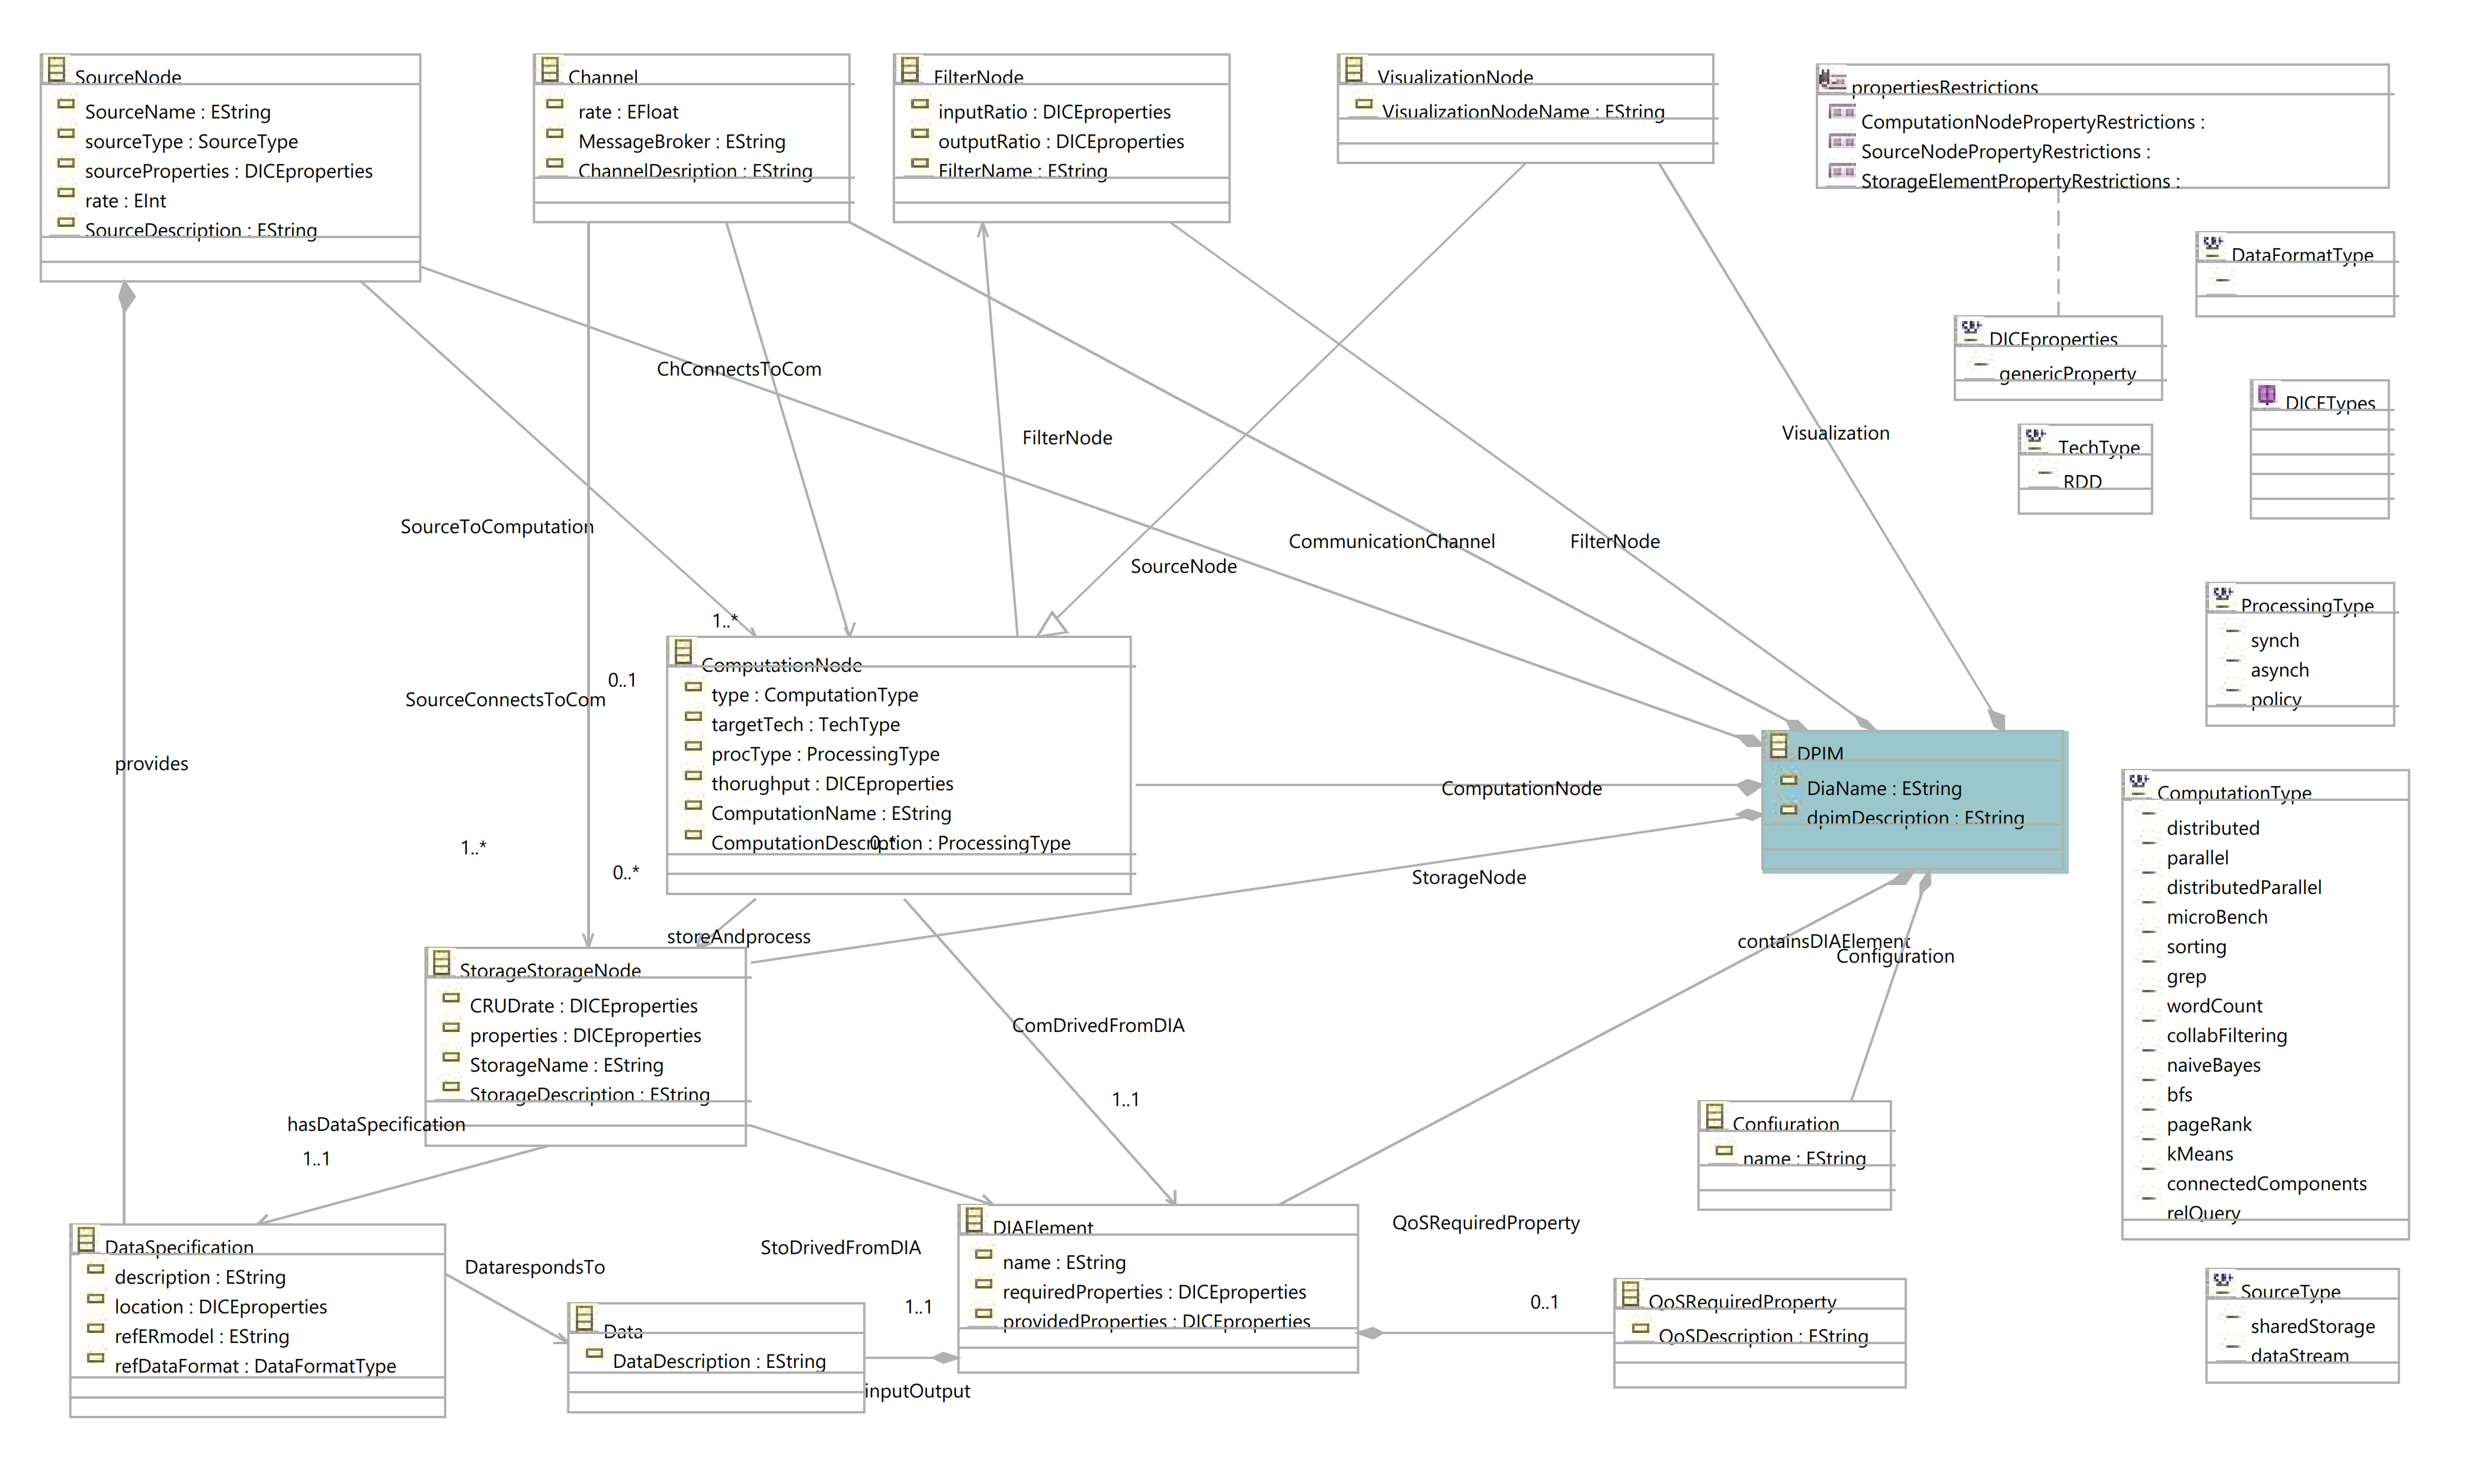
\includegraphics[width=\textwidth]{Images/11.png}
%\caption{\label{fig:metamodel}DICE DPIM metamodel.}
%\end{sidewaysfigure}

%\begin{figure}
%\centering
%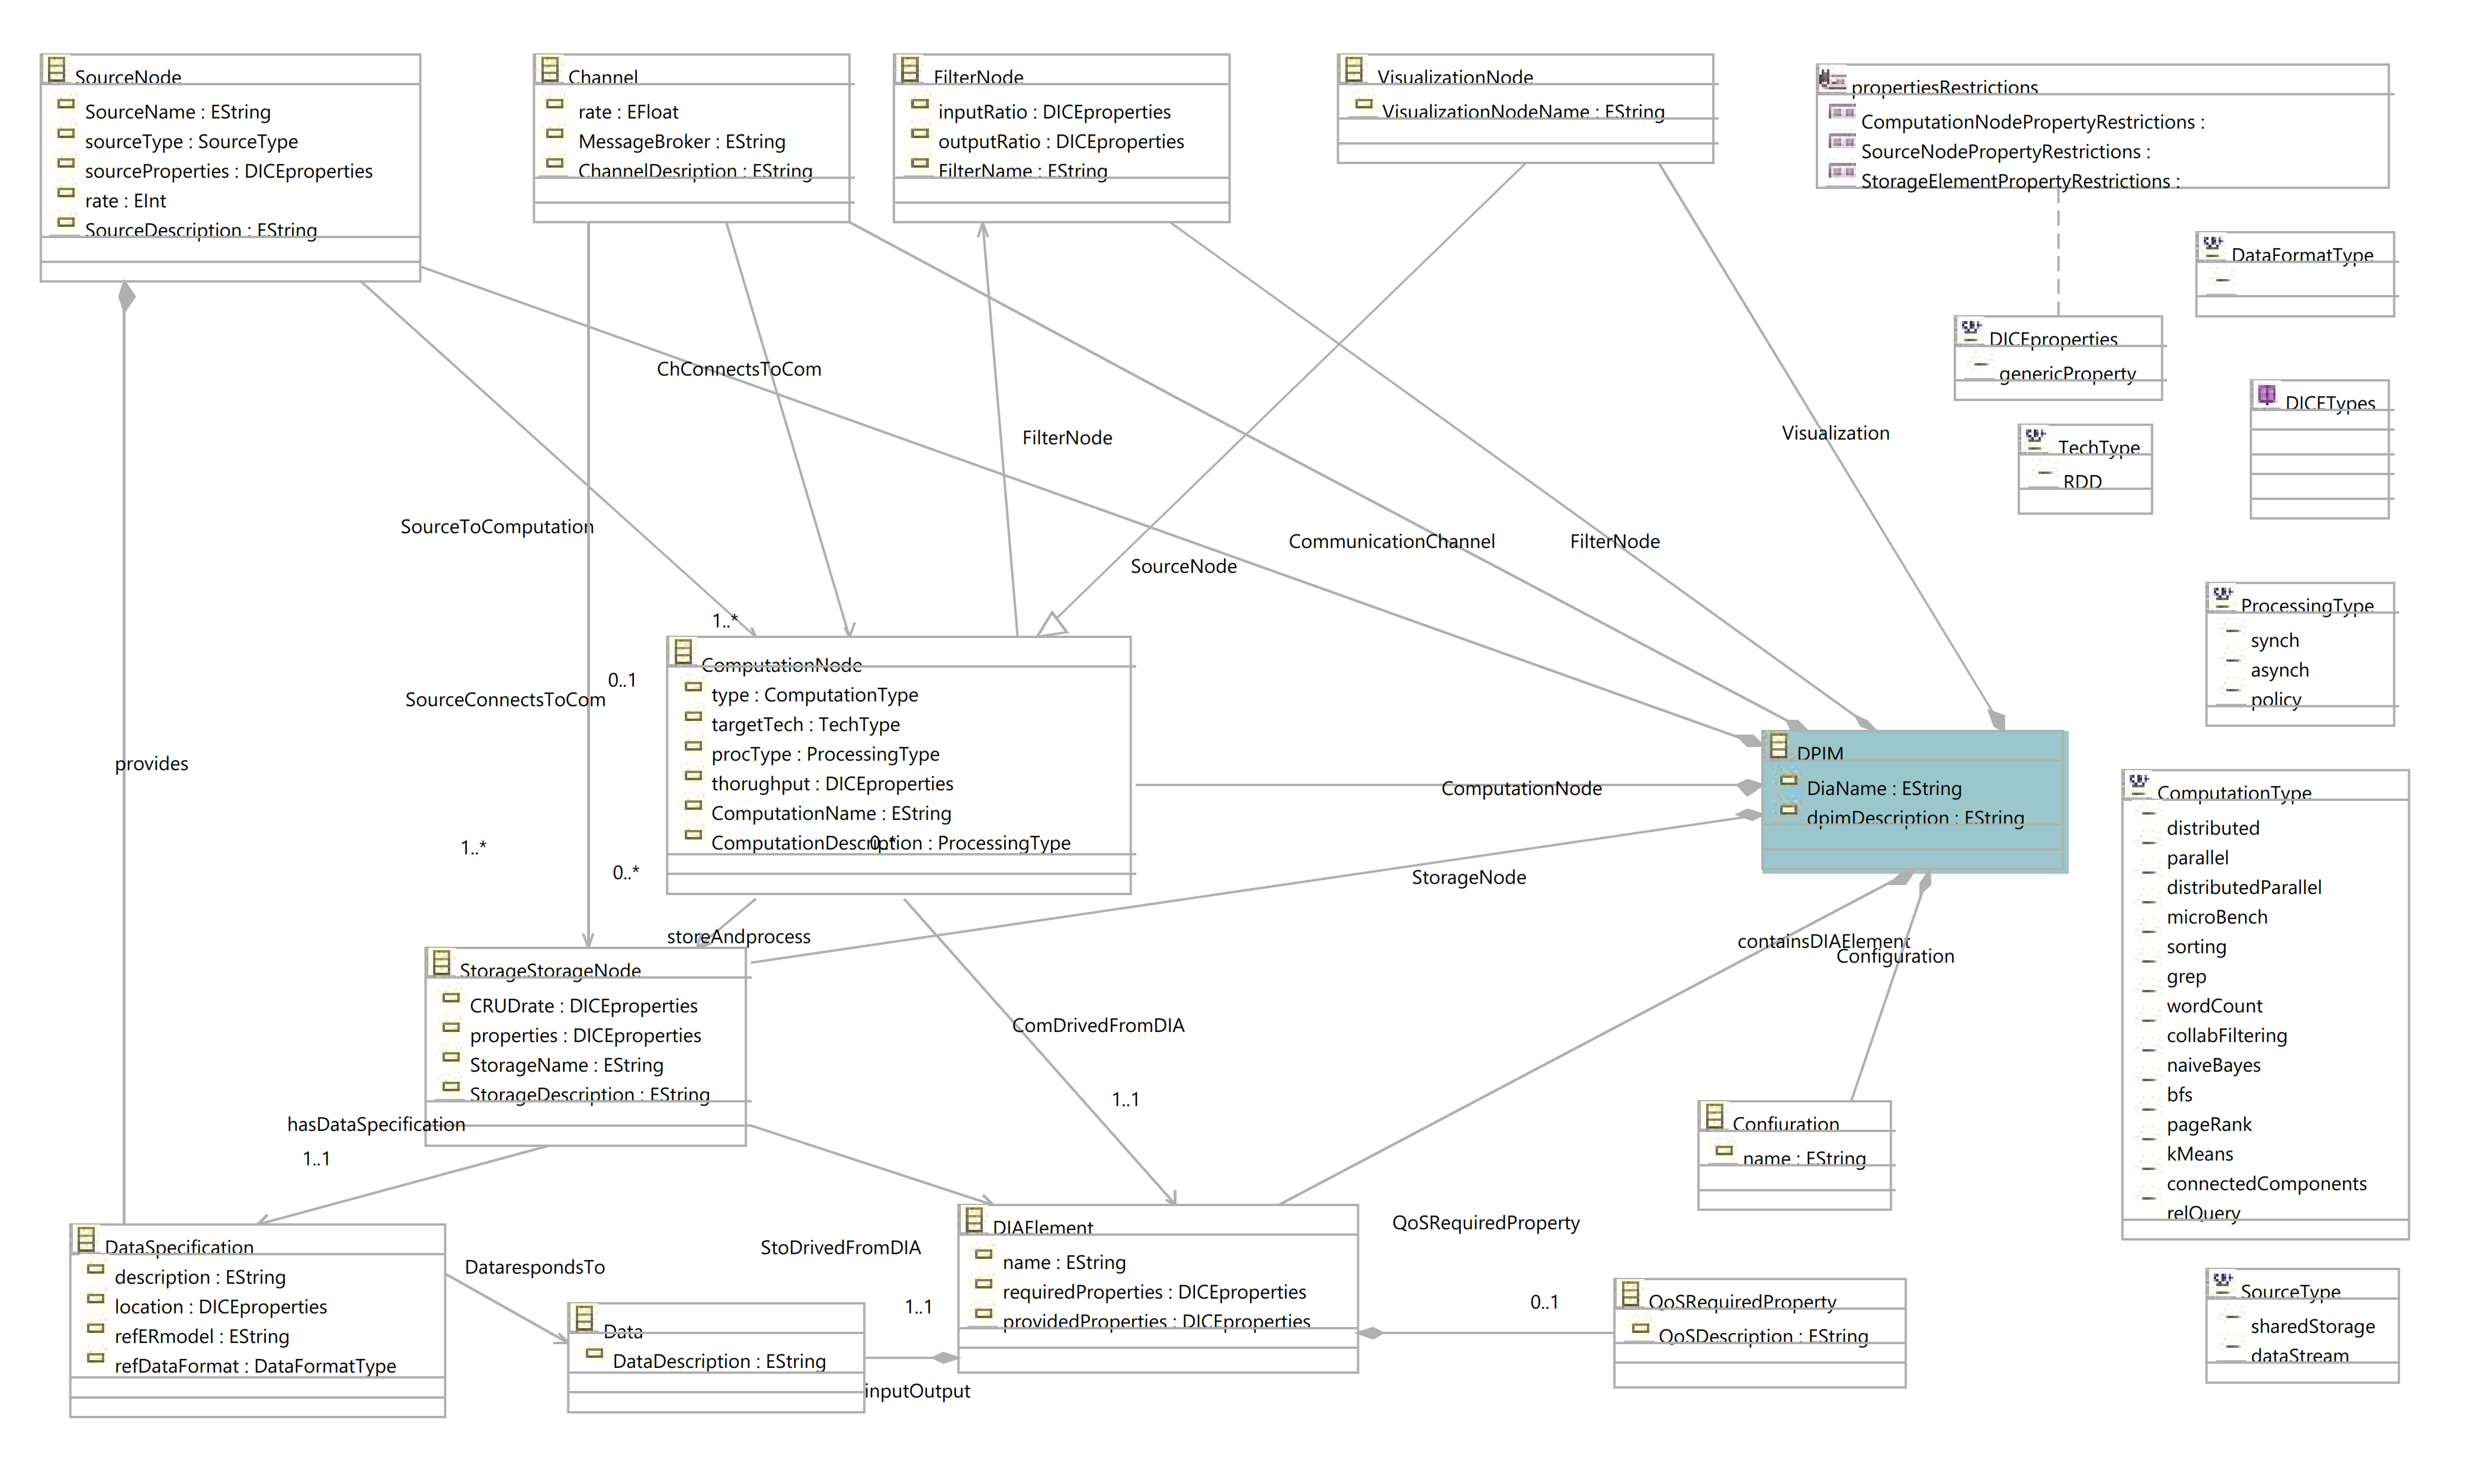
\includegraphics[width=\textwidth]{Images/11.png}
%\caption{\label{fig:metamodel2}DICE DPIM metamodel in portrait form.}
%\end{figure}

%Here is the command to refer to another element (section, figure, table, ...) in the document: \emph{As %discussed in Section~\ref{sect:overview} and as shown in Figure~\ref{fig:metamodel}, ...}. Here is how to %introduce a bibliographic citation~\cite{DAM}. Bibliographic references should be included in a \texttt{.bib} file. 

%Table generation is a bit complicated in Latex. You will soon become proficient, but to start you can %rely on tools or external services. See for instance this \href{https://www.tablesgenerator.com}{https://%www.tablesgenerator.com}. 

% -----------------------------------------------------
\subsection{Product perspective}

    \subsubsection{Scenarios} 
    
        \begin{enumerate}
            
            % - 1 -
            \item \textbf{A student wants to start using the Students\&Companies website}:
            \\Bob is a university student that is looking for an internship to enhance his CV and he decides to exploit a website to facilitate the research, so he connects to S\&C. After entering to the platform for the first time he must register himself on the web application; therefore, he selects the option \textit{"Register as student"} and he fills out sign-up form beginning the registration process providing his email, his full name and creating a password. Bob is then asked to confirm the registration using a link sent on his mailbox and, following the URL, the confirmation is done. At this point Bob will be able to fill out all the information required to complete the account such as \textit{Basic Information}, \textit{Academic Information}, and \textit{Skills and Expertise} (like technical skills, soft skills, and certifications). Bob can also include \textit{Experience and Achievements}, \textit{Internship Preferences}, \textit{CV}, \textit{Portfolio/Projects}, and \textit{Languages Spoken}. Until Bob fills out all the required information he will not be able to use the platform.
            
            % - 2 -
            \item \textbf{A student changes his personal information}:
            \\ Jack has finished some new projects, updated his CV and took a new certification. He logs into S\&C to update his personal information. There he can modify many fields and save the changes. 
            
            % - 3 -
            \item \textbf{A company changes his personal information}:
            \\ The company WeInnovate decides to update his profile on S\&C. On the profile page, it can make changes on the company information.  
            
            % - 4 -
            \item \textbf{A company wants to start using the Students\&Companies website}:
            \\Bridgenix is a company that is looking for interns for an internship that want to offer and it decides to exploit a website to facilitate the research, so it connects to S\&C. After entering to the platform for the first time it must register itself on the web application; therefore, it selects the option \textit{"Register as company"} and it fills out sign-up form beginning the registration process providing its company email, its name and creating a password. The enterprise is then asked to confirm the registration using a link sent on its mailbox and, following the URL, the confirmation is done. At this point Bridgenix will be able to navigate on the homepage and to access to its personal profile in which it can fill out all the information required to complete the account such as \textit{Basic Information} and \textit{Internship Program Details}. The company can also include \textit{Testimonials} from former interns or current employees, enhancing its profile by showcasing the company culture and employee experiences.
            
            % - 5 -
            \item \textbf{A company wants to post a new internship and review student applications}:
            \\After setting up its profile, Bridgenix can post available internships by navigating to the internship creation section. Here, the company can specify details in the \textit{Internship Role Description}, including the title, responsibilities, required skills, qualifications, and the application process.
            It can also provide \textit{Application Details}, to guide students on how to apply for the internship, specifying any required documents. Additionally, Bridgenix may list \textit{Perks and Benefits} associated with the position, such as compensation, additional benefits, and other perks to make the role more attractive to prospective interns. Once the company has fully set up the internship details, it can publish the opportunity on the platform. 
            Every time a student applies for the position, Bridgenix will receive a notification, allowing the company to review the application submitted. For each candidate, the enterprise can access complete details, and if is interested, initiate the selection process to begin evaluating the applicant.
            
            % - 6 -
            \item \textbf{A student proactively searches for an internship}:  
            \\Anita is a student registered to S\&C. Once she is logged into the platform, she can easily find the \textit{Available job search} button. By clicking it, the student will be redirected to another page of the website where she can type into the search bar specific keywords or she can apply specific filters on the search. After issuing the search, Anita will see a list of all the suitable internship positions with synthetic details about the company which is offering it. If she clicks one of them, she will be able to see more details on it.
            
            % - 7 -
            \item \textbf{A company looks for a match}   
            \\The company WorkInc is registered to the platform and has some open positions for internships. The person who is logged in for the company can click the button \textit{"Match Internship"} on the page of a specific internship, then the platform runs analytics to match it with as many students as possible. Internship pages feature a section \textit{"Matching Candidates"} where there is a list of all the suitable candidates for the positions. 
            
            % - 8 -
            \item \textbf{Users interact in the application process}
            \\ The company JobCo has to evaluate some selected students who applied to one of his internships. JobCo will create and upload on the platform timed or not quizzes or questions for the students. The students will submit their answer on the platform. Based on the answers JobCo will extend an offer to the best students, wait-list some others and reject all the other. The students can accept or refuse the final offer made by the company or acknowledge the fact that they were wait-listed or rejected.
            
            % - 9 -
            \item \textbf{Users keep track of the internship }
            \\ The company JobCo can leave private notes to the student, including suggestions, criticisms but also news about the internship. On the other hand, Tony, the student who is carrying out the internship, can communicate problems. Both JobCo and Tony can see the status of the internship and read information regarding the internship, that either one of the two has written on the platform.
            \item \textbf{A university wants to start using the Students\&Companies website}:
            Mordor Institute of Technology is a university that would like to monitor the internships of its students, connects to S\&C. After entering to the platform for the first time it must register itself on the web application; therefore, it selects the option \textit{"Register as university"} and it fills out sign-up form beginning the registration process providing its university email, its name and creating a password. The university is then asked to confirm the registration using a link sent on its mailbox and, following the URL, the confirmation is done
            
            \item \textbf{Universities monitor the internships of their students }
            \\ The university of Erewhon has a list of all the students enrolled to it that are doing an internship. The university can further look into the internship and getting to know the details of it (the company, the duration, location, role title, etc.). However, the university can look the status of an internship only once it is started, not before.
        \end{enumerate}
        
        \newcommand{\mycomment}[1]{}
        \mycomment{
            \begin{enumerate}[label=\textbf{[\arabic*]}, left = 0 pt, align = left]
            % ----
            \item \textbf{A Student Registers on the Platform}:             % DONE
            \\A student that is looking for an internship visits the S\&C platform for the first time. He or she decides to register to access potential internship opportunities.
            They enter the Homepage and clicks on \textit{"Sign Up"}. At this point, a form appears where the student must insert his email, creates a password, and fills in their personal and academic details. After submitting the form, they quickly receive an email confirmation and follow the link to activate their account. 
            Excited to start his search, the user logs in and begins creating his profile to make himself more visible to companies.
            
            % ----
            \item \textbf{Company Registration}:                            % DONE                     
            \\A company that is looking for interns visits the S\&C platform for the first time. It decides to register so it can access potential internship candidates. 
            It enters the Homepage and clicks on \textit{"Sign In"}. At this point a form appears where the enterprise must insert the company name, the company email and creates a password. After submitting the form, it quickly receives an email confirmation and follows the link to activate its account. 
            Excited to find the right candidates, the company logs in and begins creating its profile to make its internships more visible to prospective interns.
            
            % ----
            \item \textbf{Student Profile Creation}:                        % DONE
            \\Once a student logs into the platform, they can click on the \textit{"Edit profile"} button, which will redirect to a dedicated webpage displaying all the information required for the registration, along with a form that they can fill out. The student can add \textit{Basic Information}, \textit{Academic Information}, and \textit{Skills and Expertise} (like technical skills, soft skills, and certifications).
            They can also include \textit{Experience and Achievements}, \textit{Internship Preferences}, \textit{CV}, \textit{Portfolio/Projects}, and \textit{Languages Spoken}
            
            % ----
            \item \textbf{Company Profile Creation}:                        % DONE
            \\Once a company logs into the platform, it can access to its profile by clicking on the icon in the
            top-right corner of the screen. This directs the company to its profile page, where it can select the \textit{"Edit Profile"} button to add or modify information. Here, the company can fill details to personalize its profile, such as \textit{Basic Information} and \textit{Internship Program Details}.
            The company can also include \textit{Testimonials} from former interns or current employees, enhancing its profile by showcasing the company culture and employee experiences.
            
            % ----
            \item \textbf{Internship Posting by Company}:                   % DONE       
            \\After setting up its profile, the company can post available internships by navigating to the internship creation section. Here, it can specify \textit{Internship Role Description} details, including the role title, responsibilities, required skills and qualifications, and the application process.
            The company can also provide \textit{Application Details}, which feature an \textit{"Apply Now"} button for candidates and any required documents. It may also list \textit{Perks and Benefits} associated with the internship, such as compensation, additional benefits, and other perks to make the position more attractive to prospective interns.
            
            % ----
            \item \textbf{A Student Proactively Searches for an Internship}:  % DONE                 
            \\Anita is a student registered to S\&C. Once she is logged into the platform, he or she can easily find the \textit{"Available job search"} button. By clicking it the student will be redirected to another page of the website where they can type into the search bar specific keywords or they can apply specific filters on the search. After issuing the search, she will see a list of all the suitable internship positions with synthetic details about the company which is offering it. If she clicks it, she will be able to see more details on it.
            
            % ----
            \item \textbf{A Student Actively Searches for a Match}:     % TO SEE              
            \\Tom, a student registered to the platform, fills or updates his/her profile with his information, he or she can click the button \textit{"Match me"} on his profile. Then, the platform runs analytics to match it with as many companies as possible. Profiles of students feature a section with \textit{"Matching Internships"} where there is a list of all the suitable internships for him/her.
            
            % ----
            \item \textbf{A Company Looks for a Match}                  % DONE
            \\The company WorkInc is registered to the platform and has some open positions for internships. The person who is logged in for the company can click the button \textit{"Match Internship"} on the page of a specific internship, then the platform runs analytics to match it with as many students as possible. Internship pages feature a section \textit{"Matching Candidates"} where there is a list of all the suitable candidates for the positions.
            
            % ----
            \item \textbf{Student Application to Internship}                      
            \\Once a student finds an internship that might interest them, they can click on the preview of the placement, which will redirect to the company's private webpage. By pressing the \textit{"Apply Now"} button, a form will appear where the student must enter all the required information specified by the company. Once all the fields are completed, they can submit their application by clicking the \textit{"Submit"} button.
            
            % ----
            \item \textbf{Company Review of Student Applications}           % DONE 
            \\Once a company has posted one or more internship proposals, it will be able to see the applications submitted for each proposal by clicking on \textit{"Sent applications"}, which will redirect to a dedicated webpage displaying all the applications for a particular internship. For each application, brief information is shown on the screen, and the company can access the complete details by clicking the \textit{"More details"} button. If the company is interested to the student, it can click on \textit{"Start Selection Process"} to begin evaluating the candidate and will be prompted a calendar to indicate the available days and time slots.
            
            % ----
            \item \textbf{Student Interview Scheduling}  
            \\When a contact between a company and a student is established, the student will be able to choose one day from a list of available dates to conduct the interview.
            \item \textbf{Interview Conducted by Company}                        
            \\ Sarah, a student who was able to schedule an interview, will be asked a set of questions in a certain amount of time. The time and questions are decided by the company.
            \item \textbf{Company Selection of Candidate}                        
            \\
            \item \textbf{Internship Offer Extended to Student}                  
            \\
            \item \textbf{Internship Offer Acceptance by Student}                
            \\
            \item \textbf{Feedback Submission by Student Post-Internship}        
            \\
            \item \textbf{Feedback Submission by Company Post-Internship}        
            \\
            \item \textbf{Statistical Analysis of Internship Matches}            
            \\
            \item \textbf{Internal Status Update by Student}                     
            \\
            \item \textbf{Internship Status Update by Company}                   
            \\
            \item \textbf{Notification of New Internship Opportunities}          
            \\
            
            \end{enumerate}
        }
    
    % -----------------------------------------------------.
    \newpage
    \subsubsection{Domain Class Diagram}
    To capture the different classes, their methods and their interactions we drew the following domain class diagram
        \begin{figure}[h!]
            \centering
            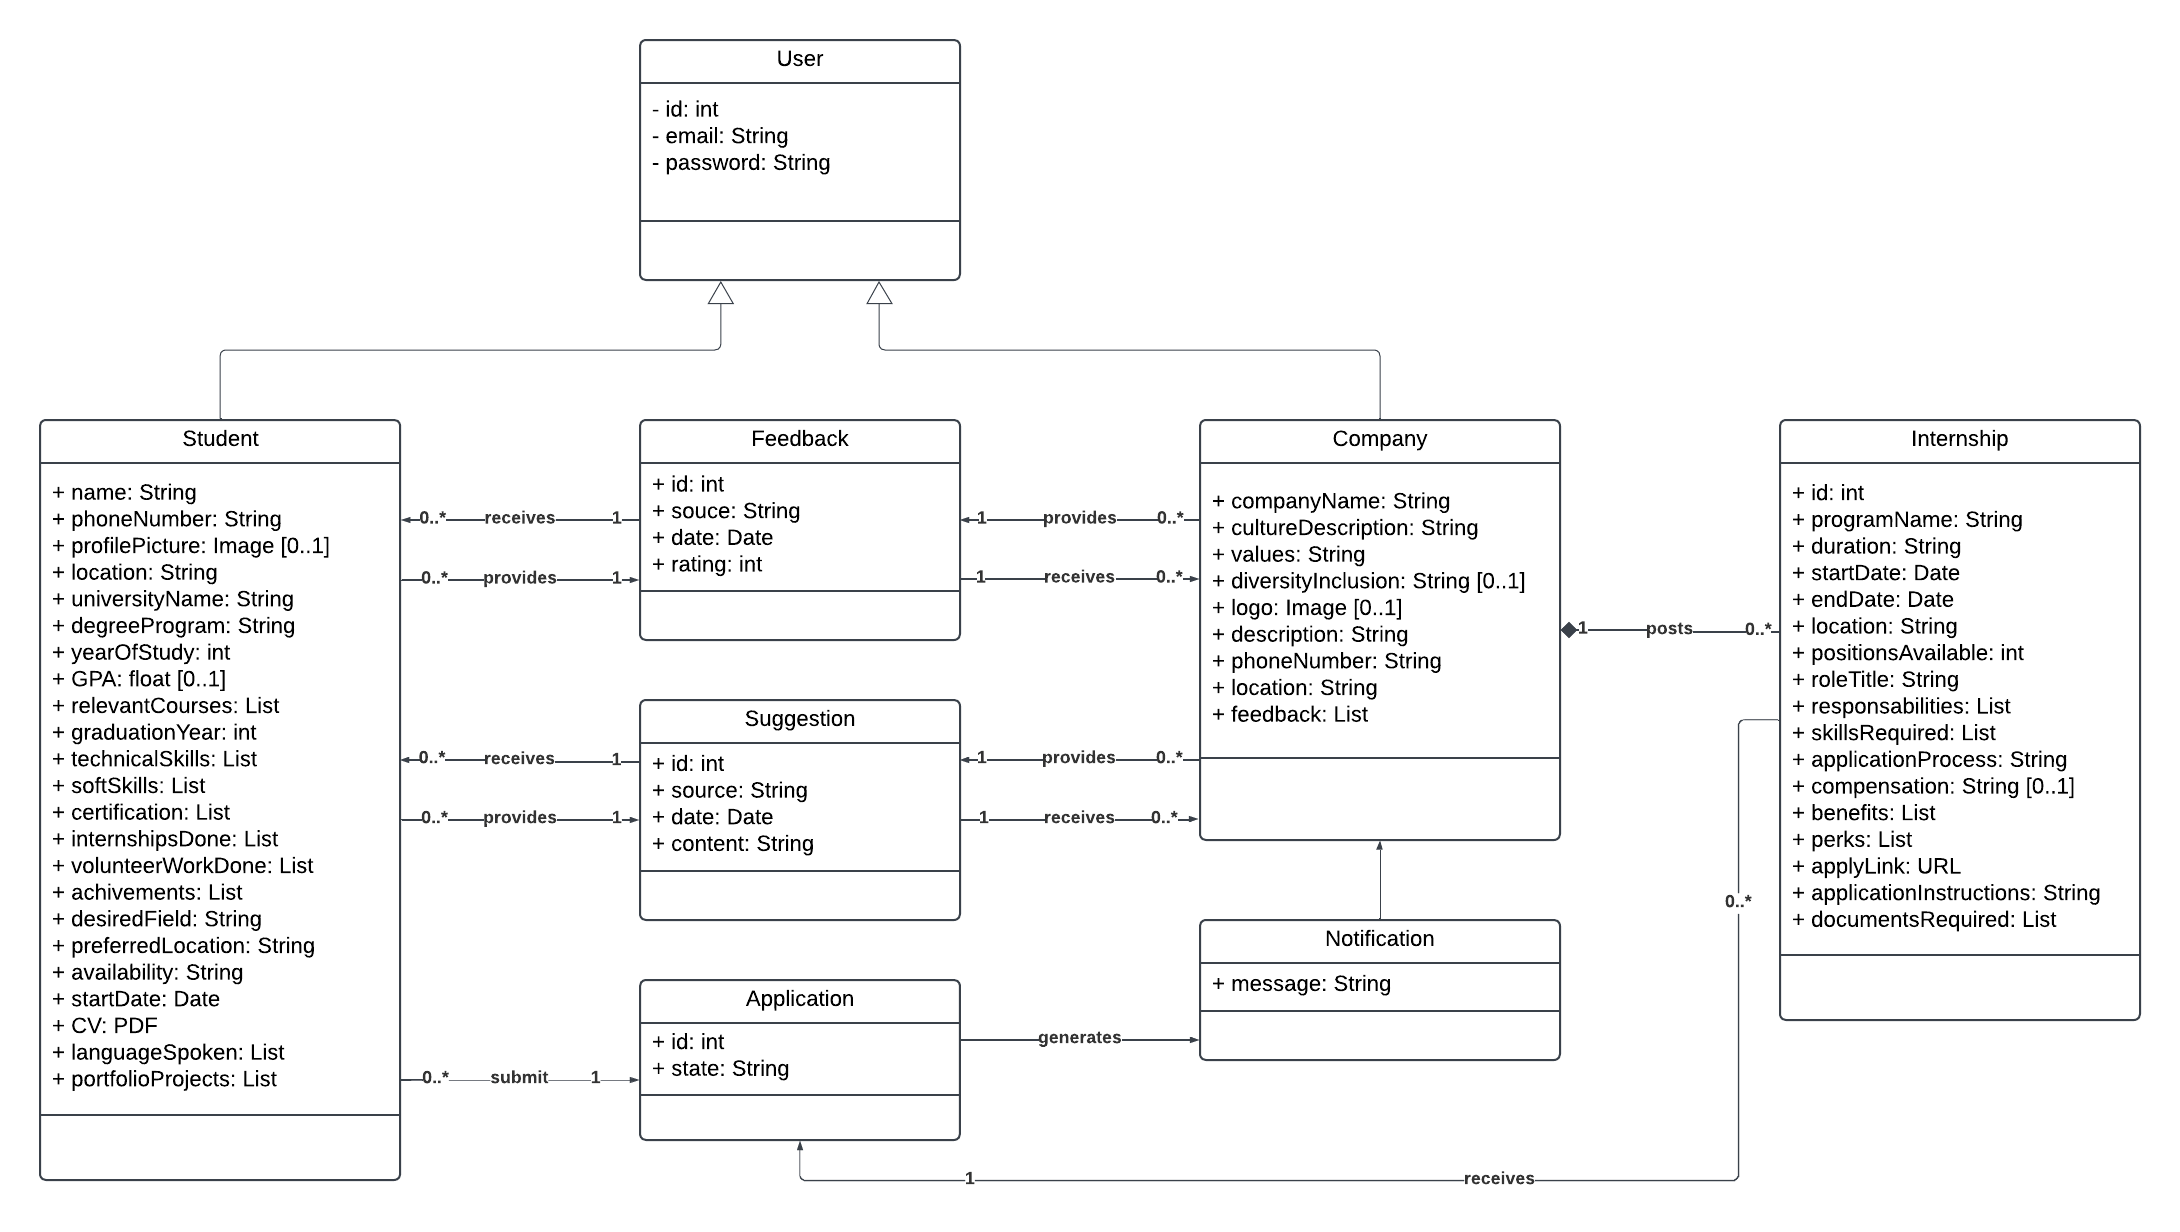
\includegraphics[width=1\textwidth]{RASD/Images/ClassDiagram.png}
            \caption{Class Diagram}
            \label{fig:example}
        \end{figure}
    
    
    % -----------------------------------------------------
    
    \subsubsection{State Diagrams}
        The most crucial aspect of the application is the creation and evolution of the internship positions on the platform. Not to leave any room for doubts, we explain both the point of view of the company and the one of the student.
        \\
        A company can close an internship position whenever it wants to. Once it closes the internship, the applications who were accepted but not confirmed or not refused, the pending applications, and the applications needing an further assessments are automatically rejected. Instead, for those who confirmed, we consider the moment of the closing of the open position by the company as the moment in which they start their internship.
        \\
        The following is the point of view of the company
        \begin{figure}[h!]
            \centering
            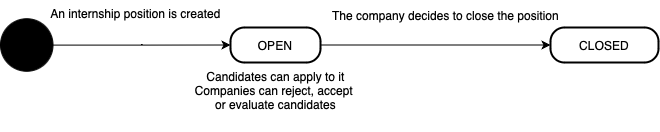
\includegraphics[width=1\textwidth]{RASD/Images/CompanyPOV.png}
            \caption{The evolution of an internship position on the platform from the point of view of a company}
            \label{fig:example}
        \end{figure}
        \\
        The following one, instead, is the point of view of a student:
        \begin{figure}[h!]
            \centering
            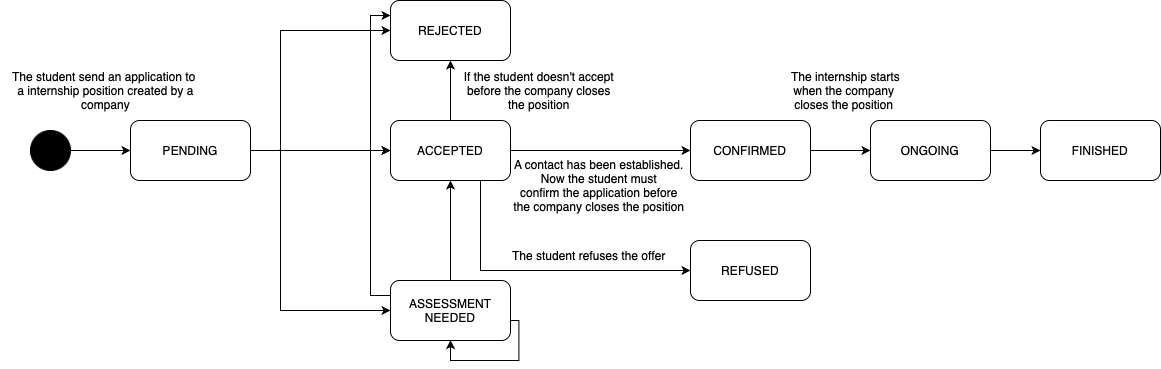
\includegraphics[width=1\textwidth]{RASD/Images/StudentPOV.png}
            \caption{The evolution of an internship position on the platform from the point of view of a student}
            \label{fig:example}
        \end{figure}
        

% -----------------------------------------------------


\subsection{Product Functions}
    \begin{enumerate}
        \item \textbf {Sign Up and Log In}
        \\ The users sign up to the platform by providing an email and a password. A registered user logs in to the platform by providing the same information. At the moment of sign up it is necessary to indicate whether the account is related to a company or to a student, since the two types of account are treated differently inside the platform.
        \item \textbf {Profile Information Filling}
        \\ The users fill his profile information. Companies will be asked for its name, the headquarters location, approximated number of employees, CEO, sector in which it operates and it can also include testimonials from former interns or current employees, showcasing the company culture and employee experiences. Students will be asked for name, surname, education, work experience, skills and CV. A part of the information is published on the platform, another part of the information is used by the recommendation system.
        \item \textbf {Internship Position Creation}
        \\ Companies can create new internships positions by establishing the expired deadline to apply, the work place, the role title, the responsibilities, the required experience, the required skills and the salary range.
        \item \textbf {Management of the Selection Process}
        \\ Companies see the profiles of students who applied to an internship. S\&C enable them to configure the selection process based on their needs. They can reject students who applied to an internship position after checking their qualifications on their profiles; they can directly accept one or more of them. Companies can propose dates of tests to assess the preparation of students who applied for an internship position and finalize the decisions after the tests or requesting an online interview.
        \item \textbf {Communication Space}
        \\ After an internship is started, both the students and companies have dedicated sections of the website to exchange information, communicate problems, indicate suggestions, make announcements (all regarding the internship) such that both of the interested parties can benefit from the sharing of information. 
        \item \textbf {Feedback Management}
        \\ After the internship is finished the platform asks both the company and the student to rate and review each other. Moreover it asks both parties for suggestions. Collecting this kind of information is particularly important to feed and improve the recommendation system.
    \end{enumerate}


% -----------------------------------------------------

\subsection{User Characteristics}
    Users of S\&C are divided into two distinct categories:


% -----------------------------------------------------

% one subsubsection for each type of user
\subsubsection{Students}
    They can search for an internship, get suggested internships, apply to open positions, participate in the selection process and give feedback about an internship for which they were selected.


% -----------------------------------------------------

\subsubsection{Companies}
    They can create internship openings, advertise them, set up the selection process, track the ongoing status of the internships and give feedback about students who undertook one of their internships.


% ------------------------------------------------------
\subsubsection{Universities}
    They can monitor the internships of their students and get details on them.
% ------------------------------------------------------
\subsection{Assumptions, Dependencies and Constraints}


% ------------------------------------------------------

\subsubsection{Regulatory Policies}
    Personal information will be processed in compliance with GDPR rules.


% ------------------------------------------------------

\subsubsection{Domain Assumptions}
    \begin{enumerate}[label={[D\arabic*]}]
        \item {Students insert correct information about their skills and experience}
        \item {Students do not cheat when taking skill assessment tests}
        \item {Students apply to jobs in countries where they have a work permit}
        \item {Students provide valuable feedback when asked for it}
        \item {Companies offer existing and legal contracts for the internships}
        \item {Companies insert correct information about the internships}
        \item {Companies periodically review information about the internship candidates}
        \item {Companies prepare proper skill assessment test to evaluate candidates}
        \item {Companies provide valuable feedback when asked for it}
        \item {Most of universities are contacted before the website is online so that most of them are already present on the platform, when the website is deployed}
    \end{enumerate}

%------------------------------------------------------------------------------------------------------------------------------------------------
\clearpage
{\color{Blue}{\section{Specific Requirements}}}
\label{sect:requirements}
%Organize this section according to the rules defined in the project description. 
% to do add notification on student registration and to post anew internship us

\subsection{External Interface Requirements}
    \subsubsection{User Interfaces}
    We prefer not to tie our design to any guidelines so early in the project, so we will probably give some snippets of the user interfaces in the DD. However, the principles that will guide our design will be clarity and minimalism. We believe that at the basis of a well working web application there must be a nice user interface. We are also convinced that being minimal and simple looking is a plus for a web application since a confusing user interface is one of the biggest reasons why users dislike a certain website and prefer another to it.

    \subsubsection{Hardware Interfaces}
    Being our project a web application there are not many hardware requirements. From the client side perspective the only request is about the size of the monitor. Indeed the website is going to be developed for desktop view exclusively. Apart of that, any laptop with a stable internet access will suffice. On the server side, any kind of setup is acceptable since our website does not have specific requirements for special computing power or similar capabilities.

    \subsubsection{Software Interfaces}
    From the perspective of software interfaces, there is only one standard requirement: the platform must be compatible with all the latest stable versions of the major web browsers
    
    \subsubsection{Communication Interfaces}
    S\&C communicates important information to users through notifications on the website.
    
    \begin{enumerate}
        \item  \textbf{Push Notifications}: notifications created when a company posted an internship or a student with the right skill set for an internship position becomes available on the platform
        \item \textbf{Real Time Notifications}: notifications created when an action is performed by a user to let him/her know that it has been successful or not
    \end{enumerate}

% --------------------------------------
\newpage
\subsection{Functional Requirements}
    The listed requirements are in the form suggested by IEEE\cite{502838}: 
    \newline
    \newline
    [Condition][Subject][Action][Object][Constraints on the Action] \\
    \subsubsection*{Users:}
        \begin{enumerate}[label=\textbf{R\arabic*}]
            \item S\&C shall allow users to sign up.                  
            \item S\&C shall allow users to fill in their profile information when signing up.
            \item S\&C shall allow users to log in.                   
            \item S\&C shall allow users to log out.                  
            \item S\&C shall allow users to update their profile information. 
            \item S\&C shall allow users to examine their own internships.
            \end{enumerate}
        
    \subsubsection*{Students:}
        \begin{enumerate}[label=\textbf{R\arabic*},resume]
            \item S\&C shall allow students to examine open internship positions. % To check
            \item S\&C shall allow students to examine their own applications.
            \item S\&C shall allow students to search for a specific kind of internship position.  
            \item S\&C shall allow students to apply for an internship position.
            \item If an internship position suitable for a student is opened, S\&C shall notify the student.
            \item When a student searches for an internship, S\&C shall list the different positions aligned with the student's profile.         
        \end{enumerate}
    
    \subsubsection*{Applications:}
        \begin{enumerate}[label=\textbf{R\arabic*},resume]
            \item If an application has been accepted by a company, S\&C shall allow the student who made the application to confirm or refuse the internship.
            \item If a company signals that it needs an assessment of the students' skills, S\&C shall allow the company to schedule an interview.
            \item After an interview has been scheduled, S\&C shall allow the student to access the link and see the date of the meeting.
            \item S\&C shall allow the students to see the status of their applications.
        \end{enumerate}
    
    \subsubsection*{Companies:}
        \begin{enumerate}[label=\textbf{R\arabic*},resume]
            \item S\&C shall allow companies to open and examine its internship positions.
            \item S\&C shall allow companies to accept or reject applications for their internship positions.
            \item S\&C shall allow companies to close internship positions.
            \item If a new profile of a student who could interest a company becomes available on the platform, S\&C shall notify the company.
        \end{enumerate}
    
    \subsubsection*{Communication during the internship:}
         \begin{enumerate}[label=\textbf{R\arabic*},resume]
            \item S\&C shall allow companies to leave private notes to students who are doing an internship with it.
            \item S\&C shall allow companies to send news about the internship to the students who participate in it.
            \item S\&C shall allow both parties to communicate problems in a specific space of the website.
        \end{enumerate}
    
    \subsubsection*{Feedback and Suggestions:}
        \begin{enumerate}[label=\textbf{R\arabic*},resume]
            \item S\&C shall allow students who took an internship with a company to rate the internship and vice versa.
            \item S\&C shall allow students who took an internship with a company to give suggestions to the company and vice versa.
            \item S\&C shall allow companies to send news about the internship to students who are carrying it out.
            \item S\&C shall allow both parties involved in an internship to make complaints in a dedicated space.
        \end{enumerate}
        
    \subsubsection*{Universities:}
        \begin{enumerate}[label=\textbf{R\arabic*},resume]
            \item S\&C shall allow universities to monitor the status of the internship of their students.
            \item S\&C shall allow universities to see details of the internships of their students.
        \end{enumerate}
        
\newpage

\subsection{Use Cases and Use Case Diagrams}

    This section is dedicated to use cases and use case diagrams. In order to be as clear as possible here is the general schema of the use cases and their links with the actors. 
\\
\\
\\
\\
\\
\\
\\
\\
\\
    \begin{figure}[h!]
                \centering
                    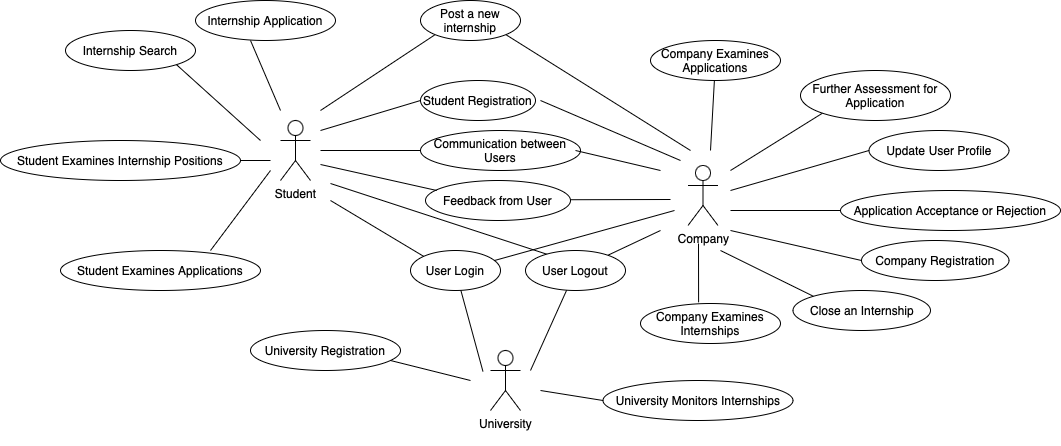
\includegraphics[width=1\textwidth]{RASD/Images/GeneralSchemaUS.drawio.png}
                \label{fig:example}
            \end{figure}
\\
\\
\\
\\
In the following pages all the use cases along with their diagrams are listed.
\newpage
    \subsubsection{User Use Cases}
    
        \begin{enumerate}[label=\textbf{[US\arabic*]}, left = 0pt, align = left]
            % -- US1 --                                                      
            \item \textbf{User Login}
            
            \begin{longtable}{|l|p{11cm}|}  
                \hline
                \textbf{Name} & 
                    \textbf{User Login} \\
                \hline
                
                \textbf{Actors} & 
                    \begin{enumerate}[label=\textbullet, itemsep=0em]
                        \item User
                    \end{enumerate} \\
                \hline
                
                \textbf{Entry Condition} & 
                    \begin{enumerate}[label=\textbullet, itemsep=0em]
                        \item The user wants to log in;
                        \item The user has an account and is on the main page of S\&C.
                    \end{enumerate} \\
                \hline
                
                \textbf{Event Flow} &
                    \begin{enumerate}[label=\arabic*., itemsep=0.2em]
                        \item The user presses the "Login" button;
                        \item S\&C redirects the user to the login page;
                        \item The user types the email in the corresponding form field;
                        \item The user types the password in the corresponding form field;
                        \item The user presses the "Log in" button;
                        \item S\&C validates the data;
                        \item S\&C redirects the user to the homepage of S\&C.
                    \end{enumerate} \\
                \hline
                
                \textbf{Exit Condition} & 
                    The user logs into his/her profile. \\
                \hline
                
                \textbf{Exceptions} &
                    \begin{enumerate}[label=\arabic*., itemsep=0.1em]
                        \item A user with the entered email doesn't exists.
                            \begin{itemize}[label=\textbullet, itemsep=0em]
                                \item In that case, S\&C will display an error message on the screen.
                            \end{itemize}
                        \item The entered password and the stored password do not match.
                            \begin{itemize}[label=\textbullet, itemsep=0em]
                                \item In that case, S\&C will display an error message on the screen.
                            \end{itemize}
                    \end{enumerate} \\
                \hline
                
            \end{longtable}

            \newpage 
            \begin{figure}[h!]
                \centering
                    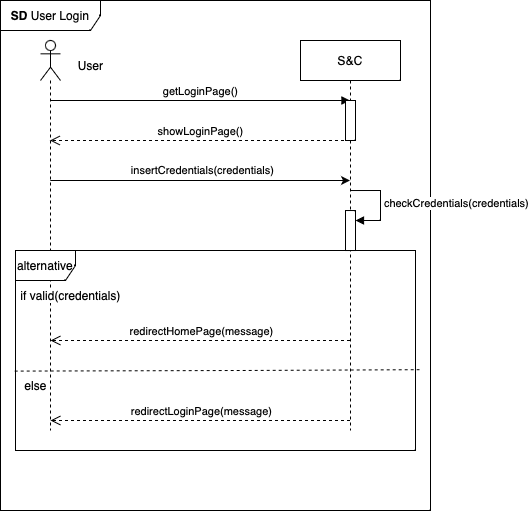
\includegraphics[width=1\textwidth]{RASD/Images/UseCases/US01_UserLogin.drawio.png}
                \label{fig:example}
            \end{figure}
  
            % -- US2 --                                                     
            \newpage
            \item \textbf{User Logout}
            
            \begin{longtable}{|l|p{11cm}|}  
                \hline
                \textbf{Name} & 
                    \textbf{User Logout} \\
                \hline
                
                \textbf{Actors} & 
                    \begin{enumerate}[label=\textbullet, itemsep=0em]
                        \item User
                    \end{enumerate} \\
                \hline
                
                \textbf{Entry Condition} & 
                    \begin{enumerate}[label=\textbullet, itemsep=0em]
                        \item The user wants to log out;
                        \item The user has an account, is logged in, and is on his/her homepage.
                    \end{enumerate} \\
                \hline
                
                \textbf{Event Flow} &
                    \begin{enumerate}[label=\arabic*., itemsep=0.2em]
                        \item The user presses the "Logout" button;
                        \item S\&C redirects the user to the login page and displays a Success Message;
                    \end{enumerate} \\
                \hline
                
                \textbf{Exit Condition} & 
                    The user logs out his/her profile. \\
                \hline
                
                \textbf{Exceptions} &
                    \begin{enumerate}[label=\arabic*., itemsep=0.1em]
                        \item The user doesn't have an account.
                            \begin{itemize}[label=\textbullet, itemsep=0em]
                                \item In that case, S\&C will display an error message on the screen.
                            \end{itemize}
                    \end{enumerate} \\
                \hline
                
            \end{longtable}

            \newpage
            \begin{figure}[h!]
                \centering
                    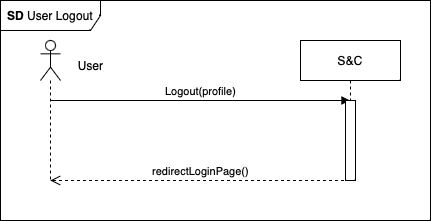
\includegraphics[width=1\textwidth]{RASD/Images/UseCases/US02_UserLogout.drawio.png}
                \label{fig:example}
            \end{figure}

            % -- US3 --                                                      
            \newpage
            
            \item \textbf{Update User Profile}
            
            \begin{longtable}{|l|p{11cm}|}  
                \hline
                \textbf{Name} & 
                    \textbf{Update User Profile} \\
                \hline
                
                \textbf{Actors} & 
                    \begin{enumerate}[label=\textbullet, itemsep=0em]
                        \item User
                    \end{enumerate} \\
                \hline

                \textbf{Entry Condition} & 
                    \begin{enumerate}[label=\textbullet, itemsep=0em]
                        \item The user decides to modify his/her profile;
                        \item The user has an account, is logged in, and is on his homepage.
                    \end{enumerate} \\
                \hline
                
                \textbf{Event Flow} &
                    \begin{enumerate}[label=\arabic*., itemsep=0.2em]
                        \item The user presses the "Edit Profile" button;
                        \item S\&C redirects the user to the personal profile page;
                        \item The user choose which information modify;
                        \item The user presses the "Modify" button on the right of the desired category;
                        \item The user modifies the data;
                        \item The user presses the "Apply Changes" button;
                        \item S\&C validates the data;
                        \item S\&C redirects the user to the homepage of S\&C.
                    \end{enumerate} \\
                \hline
                
                \textbf{Exit Condition} & 
                    The user's profile is successfully updated and saved in the system. \\
                \hline
                
                \textbf{Exceptions} &
                    \begin{enumerate}[label=\arabic*., itemsep=0.1em]
                        \item Missing Required Fields:
                            \begin{itemize}[label=\textbullet, itemsep=0em]
                                \item If any mandatory fields are left empty, S\&C will display an error message.
                            \end{itemize}
                        \item Invalid Data Format:
                            \begin{itemize}[label=\textbullet, itemsep=0em]
                                \item If at least one data is invalid, an error message is displayed;
                            \end{itemize}     
                    \end{enumerate} \\
                \hline
                
            \end{longtable}
        
            \newpage          
            \begin{figure}[h!]
                \centering
                    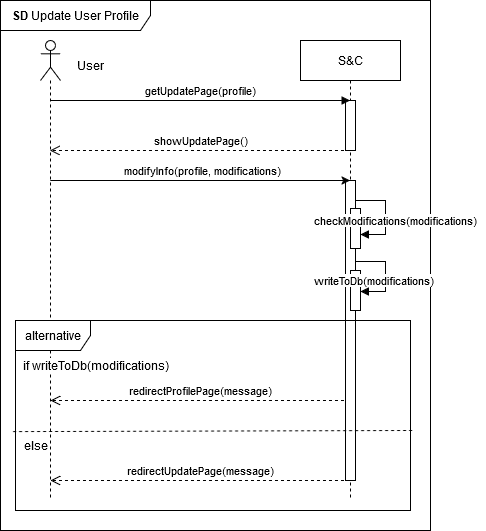
\includegraphics[width=1\textwidth]{RASD/Images/UseCases/US03_UserUpdate.drawio.png}
                \label{fig:example}
            \end{figure}

        \end{enumerate}

    % -----------------------------------
    \newpage
    \subsubsection{Student Use Cases}
    
        \begin{enumerate}[label=\textbf{[US\arabic*]}, left = 0pt, align = left, resume]
            % -- US4 --    
            \item \textbf{Student Registration}
            
            \begin{longtable}{|l|p{11cm}|}  
                \hline
                \textbf{Name} & 
                    \textbf{Student Registration} \\
                \hline
                
                \textbf{Actors} & 
                    \begin{enumerate}[label=\textbullet, itemsep=0em]
                        \item Student;
                        \item Company.
                    \end{enumerate} \\
                \hline
                
                \textbf{Entry Condition} & 
                    The student does not have an account and is on the main page of S\&C. \\
                \hline
                
                \textbf{Event Flow} &
                    \begin{enumerate}[label=\arabic*., itemsep=0.2em]
                        \item The student presses the "Register as Student" button;
                        \item S\&C redirects the student to the register page;
                        
                        \item The student types the Email in the corresponding form field;
                        \item The student types the password in the corresponding form field;
                        \item The student types the confirm password in the corresponding form field;
                        
                        \item The student enters the \textit{Basic Information} in the corresponding form field:
                        \begin{itemize}[label=\textbullet, itemsep=0em]
                            \item Full name;
                            \item Phone number;
                            \item Profile picture (not mandatory);
                            \item Location for location-based internships.
                        \end{itemize}
                        
                        \item The student enters the \textit{Academic Information}:
                        \begin{itemize}[label=\textbullet, itemsep=0em]
                            \item University name;
                            \item Degree program;
                            \item GPA (not mandatory);
                            \item Graduation year (not mandatory).
                        \end{itemize}
                        
                        \item The student types the Skills;
                        \item The student uploads the \textit{CV};
                        \item The student types the \textit{Languages Spoken}.
                        
                        \item The student presses the "Subscribe" button;
                        \item S\&C validates the data;
                        \item S\&C creates the student's account;
                        \item S\&C redirects the student to the homepage of S\&C.
                        \item S\&C identifies the internships that match the student's profile based on skills, academic background, and location;
                        \item S\&C sends notifications to companies offering internships that match the student's profile.
                    \end{enumerate} \\
                \hline
                
                \textbf{Exit Condition} & 
                    The student's account is created, and they are logged in. \\
                \hline
                
                \textbf{Exceptions} &
                    \begin{enumerate}[label=\arabic*., itemsep=0.1em]
                        \item The student provides invalid data (e.g., invalid email format, duplicate email address, mismatched passwords).
                            \begin{itemize}[label=\textbullet, itemsep=0em]
                                \item S\&C validates the input and detects the invalid data.
                                \item S\&C displays an error message explaining the specific validation errors.
                                \item The student must correct the errors and resubmit the form
                            \end{itemize}
                    \end{enumerate} \\
                \hline
            \end{longtable}
            
            \newpage
            \begin{figure}[h!]
                \centering
                    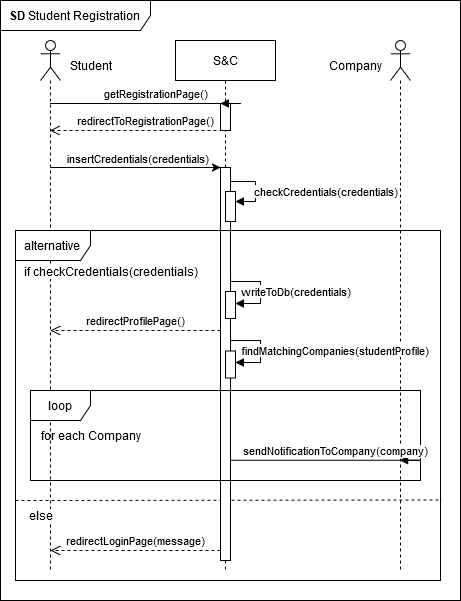
\includegraphics[width=1\textwidth]{RASD/Images/UseCases/US04_StudentRegistration.drawio.png}
                \label{fig:example}
            \end{figure}           
            
            % -- US5 --
            \newpage
            \item \textbf{Internship Search}
            
            \begin{longtable}{|l|p{11cm}|}  
                \hline
                \textbf{Name} & 
                    \textbf{Internship Search} \\
                \hline
                
                \textbf{Actors} & 
                    \begin{enumerate}[label=\textbullet, itemsep=0em]
                        \item Student
                    \end{enumerate} \\
                \hline
               
                \textbf{Entry Condition} & 
                    \begin{enumerate}[label=\textbullet, itemsep=0em]
                        \item The student knows the search criteria;
                        \item The student has an account and is logged in.
                    \end{enumerate} \\
                \hline
                
                \textbf{Event Flow} &
                    \begin{enumerate}[label=\arabic*., itemsep=0.2em]
                        \item The student clicks on the "Search" button
                        \item S\&C redirects the student to the search page;
                        \item The student searches for keyword or compiles some filters options;
                        \item The student issues the search
                        \item S\&C looks for the results and shows them with a preview for each internship;
                        \item The student can now scroll the list of internships that match the search criteria;
                        \item If the student is interested in any of the shown positions can click to discover more about it;
                        %\item Included use case: Application for internship
                    \end{enumerate} \\
                \hline
                
                \textbf{Exit Condition} & 
                    The user leaves the search page by clicking any button redirecting him or her to another page of the website \\
                \hline
                
                \textbf{Exceptions} &
                    \begin{enumerate}[label=\arabic*., itemsep=0.1em]
                        \item The criteria do not match any open position
                            \begin{itemize}[label=\textbullet, itemsep=0em]
                                \item In that case, S\&C will show a notification on the screen saying that no open position matched the search criteria
                            \end{itemize}
                        \item One or more keywords entered are not valid.
                            \begin{itemize}[label=\textbullet, itemsep=0em]
                                \item In that case, S\&C will display an empty list and a warning message on the screen saying that the input keywords don't exist.
                            \end{itemize}
                    \end{enumerate} \\
                \hline
            \end{longtable}
            
            \newpage        
            \begin{figure}[h!]
                \centering  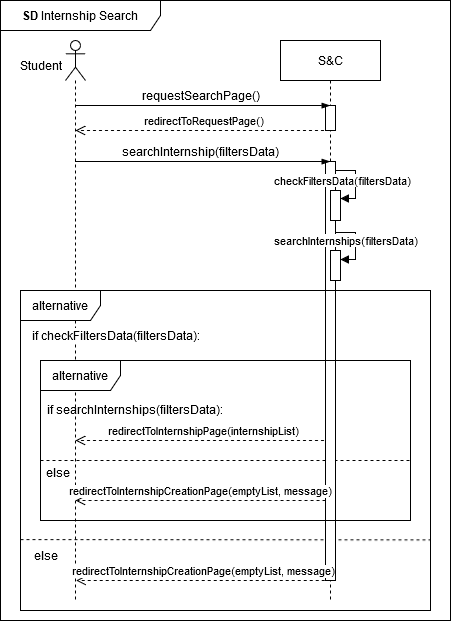
\includegraphics[width=1\textwidth]{RASD/Images/UseCases/US05_InternshipSearch.drawio.png}
                \label{fig:CompleteStudentProfile}
            \end{figure}
            
            % -- US6 --
            \newpage
            \item \textbf{Application for internship}
            
            \begin{longtable}{|l|p{11cm}|}  
                \hline
                \textbf{Name} & 
                    \textbf{Application for Internship} \\
                \hline
                
                \textbf{Actors} & 
                    \begin{enumerate}[label=\textbullet, itemsep=0em]
                        \item Student
                    \end{enumerate} \\
                \hline
                
                \textbf{Entry Condition} & 
                    \begin{enumerate}[label=\textbullet, itemsep=0em]
                        \item The student decides to apply to an internship;
                        \item The student has an account and is logged in;
                        \item The student searched an internship and he/she is on the dedicated page.
                    \end{enumerate} \\
                \hline
                
                \textbf{Event Flow} &
                    \begin{enumerate}[label=\arabic*., itemsep=0.2em]
                        \item The student presses the "Apply" button;
                        \item S\&C redirects the student to the page of the internship position;
                        \item The student can see all the information
                        \item The student has to accept terms and condition of the application
                        \item The student presses the "Confirm" button
                    \end{enumerate} \\
                \hline
                
                \textbf{Exit Condition} & 
                    The user sent the application and gets redirected to his own profile page\\
                \hline
                
                \textbf{Exceptions} &
                    \begin{enumerate}[label=\arabic*., itemsep=0.1em]
                        \item The application is made to an internship position who closed in the meanwhile but the front end has not yet rendered the change.
                            \begin{itemize}[label=\textbullet, itemsep=0em]
                                \item In that case, S\&C will display  warning message on the screen saying that the internship is not available.
                            \end{itemize}
                    \end{enumerate} \\
                \hline
            \end{longtable}
    
            \newpage
            \begin{figure}[h!]
                \centering   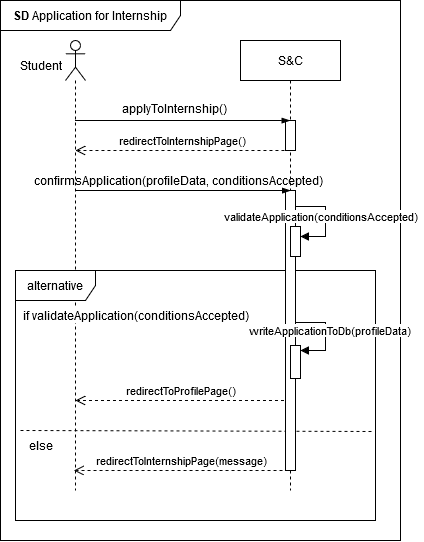
\includegraphics[width=1\textwidth]{RASD/Images/UseCases/US06_InternshipApplication.drawio.png}
                \label{fig: Application for Internship}
            \end{figure}

            % -- US7 --
            \newpage
            \item \textbf{Student Examines Applications} 
            \begin{longtable}{|l|p{11cm}|}  
                \hline
                \textbf{Name} & 
                    \textbf{Student Examines Applications} \\
                \hline
                
                \textbf{Actors} & 
                    \begin{enumerate}[label=\textbullet, itemsep=0em]
                        \item Student
                    \end{enumerate} \\
                \hline
                
                \textbf{Entry Condition} & 
                    \begin{enumerate}[label=\textbullet, itemsep=0em]
                        \item The student decides to examine its applications;
                        \item The student has an account and is logged in;
                        \item The student is on its profile page.
                    \end{enumerate} \\
                \hline
                
                \textbf{Event Flow} &
                    \begin{enumerate}[label=\arabic*., itemsep=0.2em]
                        \item The student presses the "Applications" button;
                        \item S\&C redirects the student to the page of the applications;
                        \item The student can click on any of them to get more details
                    \end{enumerate} \\
                \hline
                
                \textbf{Exit Condition} & 
                    The student exits his own profile page or confirms an application\\
                \hline
                
                \textbf{Exceptions} &
                    \begin{enumerate}[label=\arabic*., itemsep=0.1em]
                        \item The student doesn't have any applications
                            \begin{itemize}[label=\textbullet, itemsep=0em]
                                \item In that case, S\&C will display an empty list and a warning message on the screen saying that the student has not made any applications yet.
                            \end{itemize}
                    \end{enumerate} \\
                \hline
            \end{longtable}

            \newpage
            \begin{figure}[h!]
                \centering  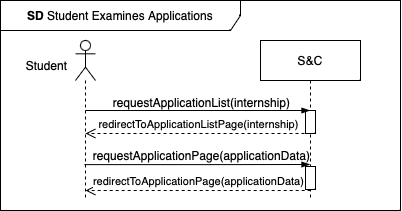
\includegraphics[width=1\textwidth]{RASD/Images/UseCases/US07_StudentExaminesApplications.drawio.png}
                \label{fig:example}
            \end{figure}
        \end{enumerate}

    % -----------------------------------
    \newpage
    \subsubsection{Company Use Cases}
        \begin{enumerate}[label=\textbf{[US\arabic*]}, left = 0pt, align = left, resume]
            % -- US8 --    
            \item \textbf{Company Registration}
        
            \begin{longtable}{|l|p{11cm}|}  
                \hline
                \textbf{Name} & 
                    \textbf{Company Registration} \\
                \hline
                
                \textbf{Actors} & 
                    \begin{enumerate}[label=\textbullet, itemsep=0em]
                        \item Company
                    \end{enumerate} \\
                \hline
                
                \textbf{Entry Condition} & 
                    The company does not have an account and is on the main page of S\&C. \\
                \hline
                
                \textbf{Event Flow} &
                    \begin{enumerate}[label=\arabic*., itemsep=0.2em]
                        \item The company presses the "Register as Company" button;
                        \item S\&C redirects the company to the register page;

                        \item The company enters the following information in the corresponding form field:
                        \begin{itemize}[label=\textbullet, itemsep=0em]
                            \item Company mail;
                            \item Password;
                            \item Confirm password
                            \item Company name;
                            \item Logo (not mandatory);
                            \item Short description of the company;
                            \item Location.
                        \end{itemize}
                        
                        \item The company presses the "Subscribe" button;
                        \item S\&C validates the data;
                        \item S\&C creates the company's account;
                        \item S\&C redirects the company to the homepage of S\&C.
                    \end{enumerate} \\
                \hline
                
                \textbf{Exit Condition} & 
                    The company's account is created, and it's logged in. \\
                \hline
                
                \textbf{Exceptions} &
                    \begin{enumerate}[label=\arabic*., itemsep=0.1em]
                        \item The company provides invalid data (e.g., invalid email format, duplicate email address, mismatched passwords).
                            \begin{itemize}[label=\textbullet, itemsep=0em]
                                \item S\&C validates the input and detects the invalid data.
                                \item S\&C displays an error message explaining the specific validation errors.
                                \item The company must correct the errors and resubmit the form.
                            \end{itemize}
                    \end{enumerate} \\
                \hline
                
            \end{longtable}

            \newpage
            \begin{figure}[h!]
                \centering  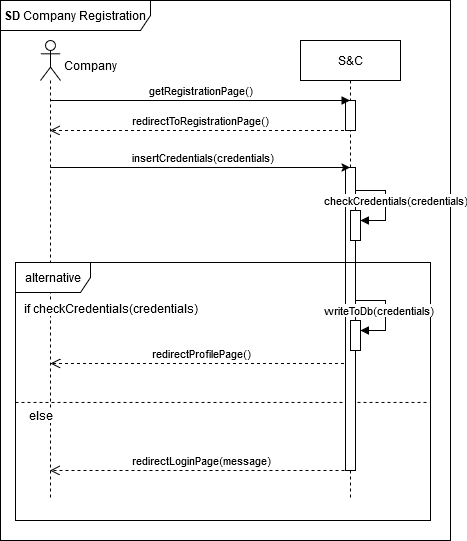
\includegraphics[width=1\textwidth]{RASD/Images/UseCases/US08_CompanyRegistration.drawio.png}
                \label{fig:CompanyRegistration}
            \end{figure}

            % -- US9 --
            \newpage
            \item \textbf{Post a new Internship}
            
            \begin{longtable}{|l|p{11cm}|}  
                \hline
                \textbf{Name} & 
                    \textbf{Post a new internship} \\
                \hline
                
                \textbf{Actors} & 
                    \begin{enumerate}[label=\textbullet, itemsep=0em]
                        \item Company;
                        \item Student.
                    \end{enumerate} \\
                \hline
                
                \textbf{Entry Condition} & 
                    The company has an account and is logged in. \\
                \hline
                
                \textbf{Event Flow} &
                    \begin{enumerate}[label=\arabic*., itemsep=0.2em]
                        \item The company presses the "Add New Internship" button;
                        \item S\&C displays a form that the company have to fill;
                        \item The company fills the form;
                        \item The company presses the "Publish" button;
                        \item S\&C validates the data;
                        \item S\&C displays a Success Message;
                        \item S\&C redirects the company to the main page;
                        \item S\&C identifies the students' profiles that match the internship based on skills, academic background, and location;
                        \item S\&C sends notifications to students that match offering the internship.
                    \end{enumerate} \\
                \hline
                
                \textbf{Exit Condition} & 
                    The company posts a new internship. \\
                \hline
                
                \textbf{Exceptions} &
                    \begin{enumerate}[label=\arabic*., itemsep=0.1em]
                        \item The company leaves one or more mandatory fields empty.
                            \begin{itemize}[label=\textbullet, itemsep=0em]
                                \item S\&C displays an error message indicating the missing fields.
                                \item S\&C highlights the empty fields in the form.
                                \item The company is prompted to complete the form before resubmitting.
                            \end{itemize}
                        \item The company provides invalid data (e.g., incorrect date formats, non-numeric salary inputs).
                            \begin{itemize}[label=\textbullet, itemsep=0em]
                                \item S\&C validates the input and detects the invalid data.
                                \item S\&C displays an error message explaining the specific validation errors.
                                \item The company must correct the errors and resubmit the form
                            \end{itemize}
                        \item The company is not logged in.
                            \begin{itemize}[label=\textbullet, itemsep=0em]
                                \item S\&C denies access and displays an error message: "You must be logged in with a company account to perform this action."
                                \item S\&C redirects the user to the login page.
                            \end{itemize}
                        \item The company attempts to post an internship with identical details to an already existing one.
                            \begin{itemize}[label=\textbullet, itemsep=0em]
                                \item S\&C detects the duplicate entry and displays a warning: "An internship with similar details already exists. Please review your submission."
                            \end{itemize}
                    \end{enumerate} \\
                \hline
                
            \end{longtable}

            \newpage
            \begin{figure}[h!]
                \centering  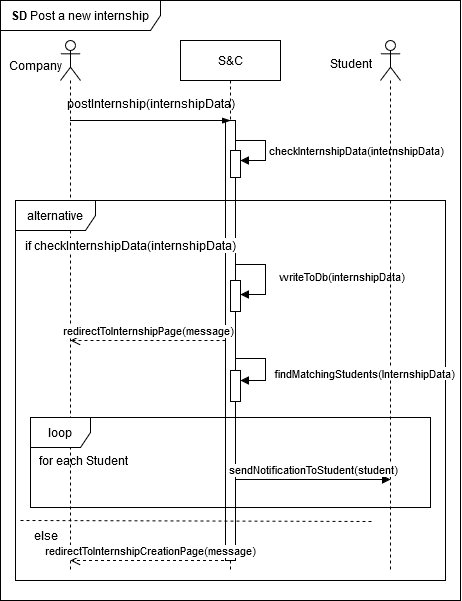
\includegraphics[width=1\textwidth]{RASD/Images/UseCases/US09_PostNewInternship.drawio.png}
                \label{fig:example}
            \end{figure}

            % -- US10 --       
            \newpage
            \item \textbf{Close an internship}
            
            \begin{longtable}{|l|p{11cm}|}  
                \hline
                \textbf{Name} & 
                    \textbf{Close an internship} \\
                \hline
                
                \textbf{Actors} & 
                    \begin{enumerate}[label=\textbullet, itemsep=0em]
                        \item Company
                    \end{enumerate} \\
                \hline
                
                \textbf{Entry Condition} & 
                    \begin{enumerate}[label=\textbullet, itemsep=0em]
                        \item The company has an account and is logged in;
                        \item The company has at least one open internship.
                    \end{enumerate} \\
                \hline 
                
                \textbf{Event Flow} &
                    \begin{enumerate}[label=\arabic*., itemsep=0.2em]
                        \item The company enters the open internship section;
                        \item The company chooses the internship they want to close;
                        \item The company presses the "Close" button;
                        \item S\&C validates the data;
                        \item S\&C displays a Success Message;
                        \item S\&C redirects the company to the main page;
                    \end{enumerate} \\
                \hline
                
                \textbf{Exit Condition} & 
                    The company posts a new internship. \\
                \hline
                
                \textbf{Exceptions} &
                    \begin{enumerate}[label=\arabic*., itemsep=0.1em]
                        \item The company is not logged in.
                            \begin{itemize}[label=\textbullet, itemsep=0em]
                                \item S\&C denies access and displays an error message: "You must be logged in with a company account to perform this action."
                                \item S\&C redirects the user to the login page.
                            \end{itemize}
                        \item The company provides invalid data (e.g., already closed internship, nonexistent internship).
                            \begin{itemize}[label=\textbullet, itemsep=0em]
                                \item S\&C validates the input and detects the invalid data.
                                \item S\&C displays an error message explaining the specific validation errors.
                            \end{itemize}
                    \end{enumerate} \\
                \hline
                
            \end{longtable}

            \newpage     
            \begin{figure}[h!]
                \centering  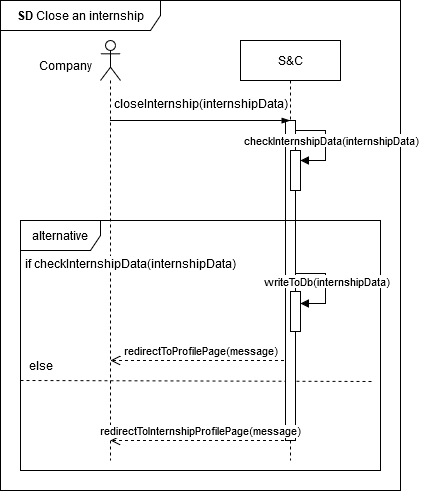
\includegraphics[width=1\textwidth]{RASD/Images/UseCases/US10_CloseInternship.drawio.png}
                \label{fig:example}
            \end{figure}
            
            % -- US11 --
            \newpage
            \item \textbf{Company Examines Internship Positions} 
            \begin{longtable}{|l|p{11cm}|}  
                \hline
                \textbf{Name} & 
                    \textbf{Company Examines Internship Positions} \\
                \hline
                
                \textbf{Actors} & 
                    \begin{enumerate}[label=\textbullet, itemsep=0em]
                        \item Company
                    \end{enumerate} \\
                \hline
                
                \textbf{Entry Condition} & 
                    \begin{enumerate}[label=\textbullet, itemsep=0em]
                        \item The company decides to examine its internship positions;
                        \item The company has an account and is logged in;
                        \item The company is on its profile page.
                    \end{enumerate} \\
                \hline
                
                \textbf{Event Flow} &
                    \begin{enumerate}[label=\arabic*., itemsep=0.2em]
                        \item The company presses the "Internships Positions" button;
                        \item S\&C redirects the company to the page of the internship positions;
                        \item The company can click on any of them to get more details;
                        \item For each internship position, the company can click on the "Candidate Matching" button;
                        \item S\&C displays a list of candidates who match the internship requirements;
                        \item The company can examine the list of candidates and review their profiles.
                    \end{enumerate} \\
                \hline
                
                \textbf{Exit Condition} & 
                    The company exits his own profile page or goes checking out some applications\\
                \hline
                
                \textbf{Exceptions} &
                    \begin{enumerate}[label=\arabic*., itemsep=0.1em]
                        \item The company doesn't have any  internship positions
                            \begin{itemize}[label=\textbullet, itemsep=0em]
                                \item In that case, S\&C will display an empty list and a warning message on the screen saying that the company has not  any internship positions yet.
                            \end{itemize}
                    \end{enumerate} \\
                \hline
            \end{longtable}

            \newpage
            \begin{figure}[h!]
                \centering
                    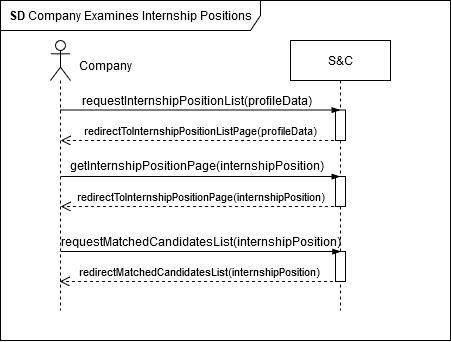
\includegraphics[width=1\textwidth]{RASD/Images/UseCases/US11_CompanyExaminesInternshipPositions.drawio.png}
                \label{fig:example}
            \end{figure}
            \newpage     

            % -- US12 --
            \newpage
            \item \textbf{Company Examines Internships} 
            
            \begin{longtable}{|l|p{11cm}|}  
                \hline
                \textbf{Name} & 
                    \textbf{Company Examines Internships} \\
                \hline
                
                \textbf{Actors} & 
                    \begin{enumerate}[label=\textbullet, itemsep=0em]
                        \item Company
                    \end{enumerate} \\
                \hline
                
                \textbf{Entry Condition} & 
                    \begin{enumerate}[label=\textbullet, itemsep=0em]
                        \item The company decides to examine its internships;
                        \item The company has an account and is logged in;
                        \item The company is on its profile page.
                    \end{enumerate} \\
                \hline
                
                \textbf{Event Flow} &
                    \begin{enumerate}[label=\arabic*., itemsep=0.2em]
                        \item The company presses the "Internships" button;
                        \item S\&C redirects the company to the page of the internships;
                        \item The company can click on any of them to get more details
                    \end{enumerate} \\
                \hline
                
                \textbf{Exit Condition} & 
                    The company exits his own profile page \\
                \hline
                
                \textbf{Exceptions} &
                    \begin{enumerate}[label=\arabic*., itemsep=0.1em]
                        \item The company doesn't have any  internships
                            \begin{itemize}[label=\textbullet, itemsep=0em]
                                \item In that case, S\&C will display an empty list and a warning message on the screen saying that the company has not  any internships yet.
                            \end{itemize}
                    \end{enumerate} \\
                \hline
            \end{longtable}

            \newpage
            \begin{figure}[h!]
                \centering  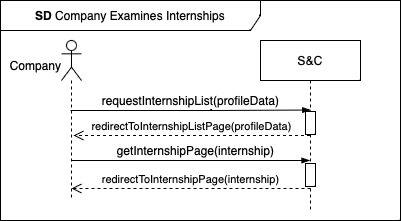
\includegraphics[width=1\textwidth]{RASD/Images/UseCases/US12_CompanyExaminesInternships.drawio.png}
                \label{fig:example}
            \end{figure}

            % -- US13 --
            \newpage
            \item \textbf{Company Examines Applications} 
            
            \begin{longtable}{|l|p{11cm}|}  
                \hline
                \textbf{Name} & 
                    \textbf{Company Examines Applications} \\
                \hline
                
                \textbf{Actors} & 
                    \begin{enumerate}[label=\textbullet, itemsep=0em]
                        \item Company
                    \end{enumerate} \\
                \hline
                
                \textbf{Entry Condition} & 
                    \begin{enumerate}[label=\textbullet, itemsep=0em]
                        \item The company decides to examine its applications;
                        \item The company has an account and is logged in;
                        \item The company is on its profile page.
                    \end{enumerate} \\
                \hline
                
                \textbf{Event Flow} &
                    \begin{enumerate}[label=\arabic*., itemsep=0.2em]
                        \item Included use case: Company Examines Internship Positions 
                        \item The company presses the "Applications" button;
                        \item S\&C redirects the company to the page of the applications;
                        \item The company can click on any of them to get more details
                    \end{enumerate} \\
                \hline
                
                \textbf{Exit Condition} & 
                    The company exits his own profile page or accept, refuse or request an assessment an application\\
                \hline
                
                \textbf{Exceptions} &
                    \begin{enumerate}[label=\arabic*., itemsep=0.1em]
                        \item The company doesn't have any applications for an internship position
                            \begin{itemize}[label=\textbullet, itemsep=0em]
                                \item In that case, S\&C will display an empty list and a warning message on the screen saying that the company has not  any applications for that internship yet.
                            \end{itemize}
                    \end{enumerate} \\
                \hline
            \end{longtable}
            
            \newpage           
            \begin{figure}[h!]
                \centering  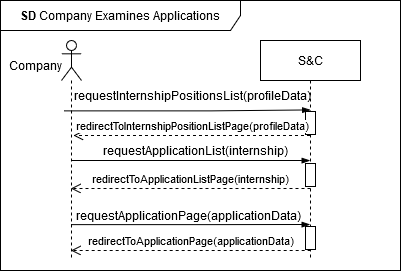
\includegraphics[width=1\textwidth]{RASD/Images/UseCases/US13_CompanyExaminesApplications.drawio.png}
                \label{fig:example}
            \end{figure}

            % -- US14 --        
            \newpage
            \item \textbf{Application Acceptance or Rejection}
            
            \begin{longtable}{|l|p{11cm}|}  
                \hline
                \textbf{Name} & 
                    \textbf{Application Acceptance or Rejection} \\
                \hline
                
                \textbf{Actors} & 
                    \begin{enumerate}[label=\textbullet, itemsep=0em]
                        \item Company
                    \end{enumerate} \\
                \hline
                
                \textbf{Entry Condition} & 
                    \begin{enumerate}[label=\textbullet, itemsep=0em]
                        \item The company has an account and is logged in;
                        \item The company knows which candidate to accept or reject; 
                        \item The company is in the dedicate page of an open internship that it has.
                    \end{enumerate} \\
                \hline
                
                \textbf{Event Flow} &
                    \begin{enumerate}[label=\arabic*., itemsep=0.2em]
                        \item The company clicks on the button to see the list of candidates;
                        \item The company can click on each item of the list to visit the profile page of the candidate;
                        \item The company clicks on the "Accept" or "Reject" button in correspondence with the candidate
                        \item S\&C displays a Success Message;
                    \end{enumerate} \\
                \hline
                
                \textbf{Exit Condition} & 
                    The candidate is accepted or rejected. \\
                \hline
                
                \textbf{Exceptions} &
                    \begin{enumerate}[label=\arabic*., itemsep=0.1em]
                        \item The company has no candidates for an open internship.
                            \begin{itemize}[label=\textbullet, itemsep=0em]
                                \item In that case, S\&C will show an empty list an display a notification which says no applications were found for that position.
                            \end{itemize}
                    \end{enumerate} \\
                \hline
            \end{longtable}

            \newpage
            \begin{figure}[h!]
                \centering  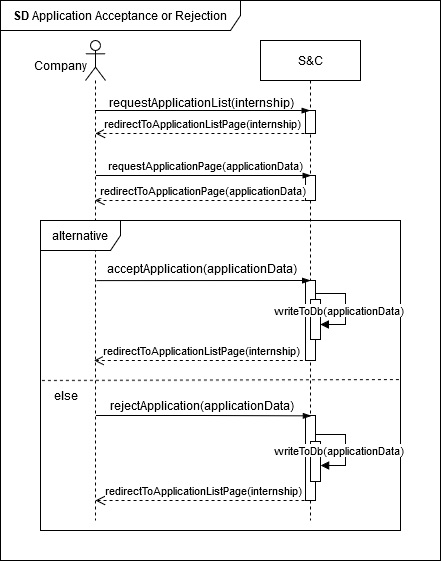
\includegraphics[width=1\textwidth]{RASD/Images/UseCases/US14_ApplicationAcceptanceRejection.drawio.png}
                \label{fig:example}
            \end{figure}

            % -- US15 --
            \newpage
            \item \textbf{Further Assessment for Application}
            
            \begin{longtable}{|l|p{11cm}|}  
                \hline
                \textbf{Name} & 
                    \textbf{Further Assessment for Application} \\
                \hline
                
                \textbf{Actors} & 
                    \begin{enumerate}[label=\textbullet, itemsep=0em]
                        \item Company
                    \end{enumerate} \\
                \hline
                
                \textbf{Entry Condition} & 
                    \begin{enumerate}[label=\textbullet, itemsep=0em]
                        \item The company has an account and is logged in;
                        \item The company knows which candidates have to undergo more assessment before being accepted or rejected;
                        \item The company is in the dedicate page of an open internship that it has.
                    \end{enumerate} \\
                \hline
                
                \textbf{Event Flow} &
                    \begin{enumerate}[label=\arabic*., itemsep=0.2em]
                        \item The company clicks on the button to see the list of candidates;
                        \item The company can click on each item of the list to visit the profile page of the candidate;
                        \item The company clicks the "Assess Further" button in correspondence with the candidate;
                        \item The company is prompted a calendar to choose when to schedule the interview and an input field to put the link of the online room;
                        \item The company confirms the date;
                        \item S\&C displays a Success Message.
                    \end{enumerate} \\
                \hline
                
                \textbf{Exit Condition} & 
                    The company has scheduled a new interview. \\
                \hline
                
                \textbf{Exceptions} &
                    \begin{enumerate}[label=\arabic*., itemsep=0.1em]
                        \item The company has no candidates for an open internship.
                            \begin{itemize}[label=\textbullet, itemsep=0em]
                                \item In that case, S\&C will show an empty list and display a notification which says no applications were found for that position.
                            \end{itemize}                           
                        \item The company inserted an invalid link.
                            \begin{itemize}[label=\textbullet, itemsep=0em]
                                \item S\&C validates the input and detects the invalid data.
                                \item S\&C displays an error message explaining the specific validation error.
                            \end{itemize}
                            
                    \end{enumerate} \\
                \hline
            \end{longtable}
            
            \newpage
            \begin{figure}[h!]
                \centering  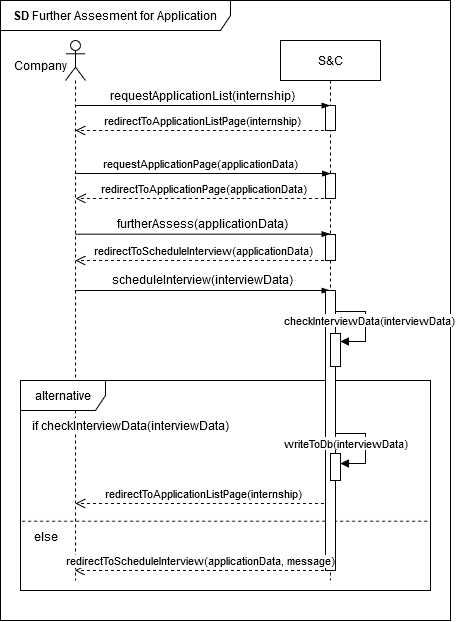
\includegraphics[width=1\textwidth]{RASD/Images/UseCases/US15_FurtherAssessment.drawio.png}
                \label{fig:example}
            \end{figure}
            
        \end{enumerate}

    % -----------------------------------
    \newpage
    \subsubsection{Users (Company and Student) Use Cases}
    Notice that in this subsection when we refer to users we intend students and companies only.
        \begin{enumerate}[label=\textbf{[US\arabic*]}, left = 0pt, align = left, resume]
            % -- US16 --
            \item \textbf{Feedback from User}
            
            \begin{longtable}{|l|p{11cm}|}  
                \hline
                \textbf{Name} & 
                    \textbf{Feedback from User} \\
                \hline
                
                \textbf{Actors} & 
                    \begin{enumerate}[label=\textbullet, itemsep=0em]
                        \item User
                    \end{enumerate} \\
                \hline
                
                \textbf{Entry Condition} & 
                    \begin{enumerate}[label=\textbullet, itemsep=0em]
                        \item The user has an account and is logged in;
                        \item The user has participated in the internship;
                        \item The internship has finished.
                    \end{enumerate} \\
                \hline
                
                \textbf{Event Flow} &
                    \begin{enumerate}[label=\arabic*., itemsep=0.2em]
                        \item The user navigates to the page of the just finished internship;
                        \item The user clicks the button to create a feedback;
                        \item The user inserts a rating and a comment;
                        \item The user sends it by clicking "Send";
                        \item S\&C validates the data;
                        \item S\&C displays a Success Message.
                    \end{enumerate} \\
                \hline
                
                \textbf{Exit Condition} & 
                    The feedback is sent and the user is redirected to the application page \\
                \hline

                \textbf{Exceptions} &
                    \begin{enumerate}[label=\arabic*., itemsep=0.1em]
                        \item The user provides invalid data (e.g., rating outside the range).
                            \begin{itemize}[label=\textbullet, itemsep=0em]
                                \item S\&C validates the input and detects the invalid data.
                                \item S\&C displays an error message explaining the specific validation errors.
                            \end{itemize}
                    \end{enumerate} \\
                \hline
            \end{longtable}

            \newpage
            \begin{figure}[h!]
                \centering  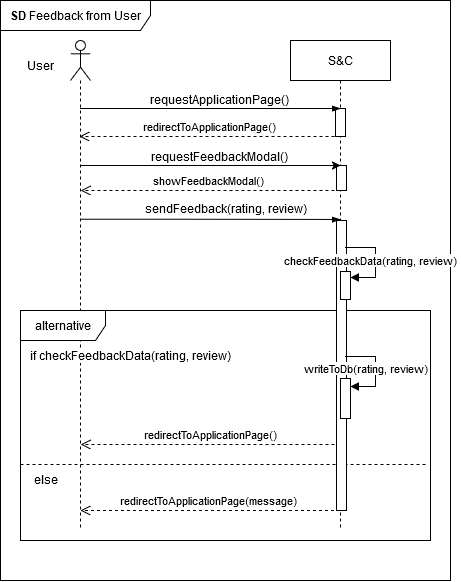
\includegraphics[width=1\textwidth]{RASD/Images/UseCases/US16_FeedbackFromUser.drawio.png}
                \label{fig:example}
            \end{figure}

            % -- US17 --
            \newpage
            \item \textbf{Communication between Users}
            
            \begin{longtable}{|l|p{11cm}|}  
                \hline
                \textbf{Name} & 
                    \textbf{Communication between Users} \\
                \hline
                
                \textbf{Actors} & 
                    \begin{enumerate}[label=\textbullet, itemsep=0em]
                        \item User
                    \end{enumerate} \\
                \hline
                
                \textbf{Entry Condition} & 
                    \begin{enumerate}[label=\textbullet, itemsep=0em]
                        \item The user has an account and is logged in;
                        \item The user is participating in the internship;
                        \item A user has to communicate something while an internship is ongoing.
                    \end{enumerate} \\
                \hline
                
                \textbf{Event Flow} &
                    \begin{enumerate}[label=\arabic*., itemsep=0.2em]
                        \item The user navigates to the page of the ongoing internship;
                        \item The user clicks the button to create a new complaint or a new suggestion;
                        \item The user inserts a message and sends it; 
                    \end{enumerate} \\
                \hline
                
                \textbf{Exit Condition} & 
                    The suggestion/complaint is sent and the student/company is redirected to the application page \\
                \hline
                \hline
            \end{longtable}

            \newpage
            \begin{figure}[h!]
                \centering  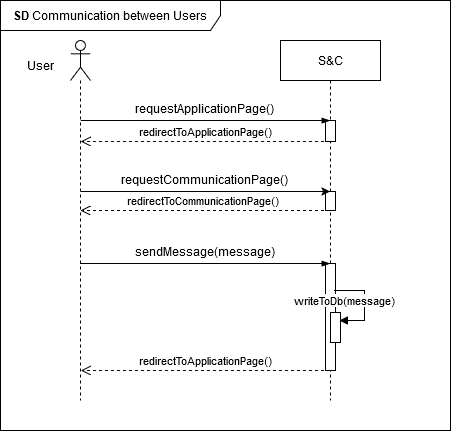
\includegraphics[width=1\textwidth]{RASD/Images/UseCases/US17_CommunicationBetweenUsers.drawio.png}
                \label{fig:example}
            \end{figure}

        \end{enumerate}

    % -----------------------------------
    \newpage
    \subsubsection{Universities Use Cases}
        \begin{enumerate}[label=\textbf{[US\arabic*]}, left = 0pt, align = left, resume]
            % -- US18 --    
            \item \textbf{University Registration}
        
            \begin{longtable}{|l|p{11cm}|}  
                \hline
                \textbf{Name} & 
                    \textbf{University Registration} \\
                \hline
                
                \textbf{Actors} & 
                    \begin{enumerate}[label=\textbullet, itemsep=0em]
                        \item University
                    \end{enumerate} \\
                \hline
                
                \textbf{Entry Condition} & 
                    The university does not have an account and is on the main page of S\&C. \\
                \hline
                
                \textbf{Event Flow} &
                    \begin{enumerate}[label=\arabic*., itemsep=0.2em]
                        \item The university presses the "Register as University" button;
                        \item S\&C redirects the university to the register page;

                        \item The university enters the following information in the corresponding form field:
                        \begin{itemize}[label=\textbullet, itemsep=0em]
                            \item University mail;
                            \item Password;
                            \item Confirm password
                            \item University name;
                            \item Address;
                            \item URL of it's website.
                        \end{itemize}
                        
                        \item The university presses the "Subscribe" button;
                        \item S\&C validates the data;
                        \item S\&C creates the university's account;
                        \item S\&C redirects the university to the homepage of S\&C.
                    \end{enumerate} \\
                \hline
                
                \textbf{Exit Condition} & 
                    The university's account is created, and it's logged in. \\
                \hline
                
                \textbf{Exceptions} &
                    \begin{enumerate}[label=\arabic*., itemsep=0.1em]
                        \item The university provides invalid data (e.g., invalid email format, duplicate email address, mismatched passwords).
                            \begin{itemize}[label=\textbullet, itemsep=0em]
                                \item S\&C validates the input and detects the invalid data.
                                \item S\&C displays an error message explaining the specific validation errors.
                                \item The university must correct the errors and resubmit the form.
                            \end{itemize}
                    \end{enumerate} \\
                \hline
                
            \end{longtable}

            \newpage
            \begin{figure}[h!]
                \centering  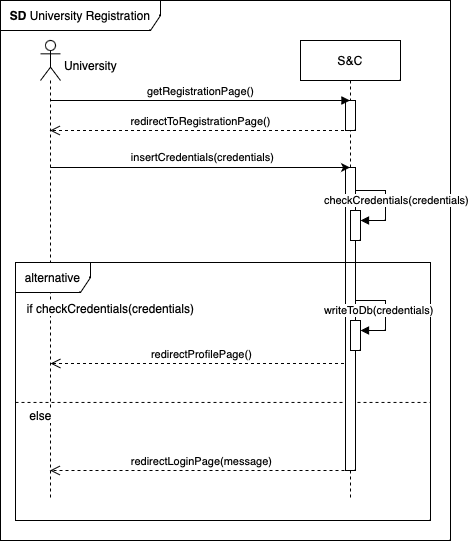
\includegraphics[width=1\textwidth]{RASD/Images/UseCases/US18_UniversityRegistration.drawio.png}
                \label{fig:example}
            \end{figure}
            
            % -- US19 --
            \newpage
            \item \textbf{University Monitors Internships}
            
            \begin{longtable}{|l|p{11cm}|}  
                \hline
                \textbf{Name} & 
                    \textbf{University Monitors Internships} \\
                \hline
                
                \textbf{Actors} & 
                    University \\
                \hline
                
                \textbf{Entry Condition} & 
                    The university is logged in \\
                \hline
                
                \textbf{Event Flow} &
                    \begin{enumerate}[label=\arabic*., itemsep=0.2em]
                        \item The university has a list of internships done by its students on its home page;
                        \item The university can click on any of them to get more details;
                    \end{enumerate} \\
                \hline
                
                \textbf{Exit Condition} & 
                    The university stops scrolling the list of hits students who got an internship  profile. \\
                \hline
                
                \textbf{Exceptions} &
                    \begin{enumerate}[label=\arabic*., itemsep=0.1em]
                        \item The universities has no students who got an internship.
                            \begin{itemize}[label=\textbullet, itemsep=0em]
                                \item In that case, S\&C will display a message on the screen saying that no enrolled student got any internship.
                            \end{itemize}
                    \end{enumerate} \\
                \hline
                
            \end{longtable}

            \newpage
            \begin{figure}[h!]
                \centering  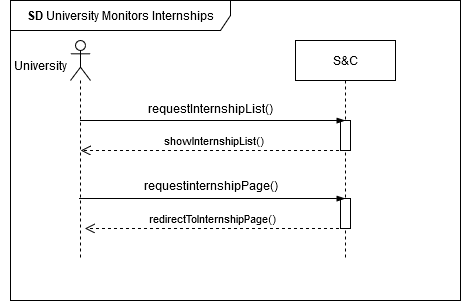
\includegraphics[width=1\textwidth]{RASD/Images/UseCases/US19_UniversityMonitorsInternships.drawio.png}
                \label{fig:example}
            \end{figure}

        \end{enumerate}
        
\newpage

\subsection{Requirement Mapping}

\begin{enumerate}[label={[G\arabic*]}]
\item \textbf{Internship Lookup for Students}: 
                Help students in their search for an internship by connecting their profiles with well-suited internship offers from companies.

\begin{longtable}{|p{8cm}|p{8cm}|}
\hline
\rowcolor[HTML]{CFE2F3} 
\textbf{Requirements} & \textbf{Mapped To} \\
\hline
\endfirsthead

\hline
\endfoot

\hline
\endlastfoot
R1 S\&C shall allow users to sign up. & D1 Students insert correct information about their skills and experience \\
R2 S\&C shall allow users to fill their profile information on sign up & D2 Students apply to jobs in countries where they have a work permit \\
R3 S\&C shall allow users to log in. & D3 Companies offer existing and legal contracts for the internships \\
R4 S\&C shall allow users to log out. & D4 Companies insert correct information about the internships \\
R5 S\&C shall allow users to update their profile information. & D5 Companies periodically review information about the internship candidates \\
R7 S\&C shall allow users to examine open internship positions.  & \\
R9 S\&C shall allow students to search for a specific kind of internship.  & \\ 
R10 S\&C shall allow students to apply for an internship.     & \\
R11 If an internship position suited to a student is opened, S\&C shall notify the student & \\
R12 When a student issues a search for an internship, S\&C shall list the different positions aligned with the student's profile.  & \\

\end{longtable}


\newpage
\item \textbf{Visibility for Internship Positions of the Companies}: 
                Allow companies to promote their internship positions to students and inform them about the availability of eligible candidates.
\begin{longtable}{|p{8cm}|p{8cm}|}
\hline
\rowcolor[HTML]{CFE2F3} 
\textbf{Requirements} & \textbf{Mapped To} \\
\hline
\endfirsthead

\hline
\endfoot

\hline
\endlastfoot
R1 S\&C shall allow users to sign up. & D1 Students insert correct information about their skills and experience \\
R2 S\&C shall allow users to fill their profile information on sign up & D2 Students apply to jobs in countries where they have a work permit \\
R3 S\&C shall allow users to log in. & D3 Companies offer existing and legal contracts for the internships \\
R4 S\&C shall allow users to log out. & D4 Companies insert correct information about the internships \\
R5 S\&C shall allow users to update their profile information. & D5 Companies periodically review information about the internship candidates \\
R7 S\&C shall allow users to examine open internship positions.  & \\
R9 S\&C shall allow students to search for a specific kind of internship.  & \\ 
R10 S\&C shall allow students to apply for an internship. & \\
R11 If an internship position suited to a student is opened, S\&C shall notify the student & \\
R12 When a student issues a search for an internship, S\&C shall list the different positions aligned with the student's profile.  & \\
R18 S\&C shall allow companies to open and examine its internship positions. & \\
\newpage
\end{longtable}
\item \textbf{Selection Process Management}: 
                Support the interaction and selection by providing a platform to companies to set up and conduct interviews, gather structured information about students and finalize the selections.

\begin{longtable}{|p{8cm}|p{8cm}|}
\hline
\rowcolor[HTML]{CFE2F3} 
\textbf{Requirements} & \textbf{Mapped To} \\
\hline
\endfirsthead

\hline
\endfoot

\hline
\endlastfoot

R1 S\&C shall allow users to sign up. & D1 Students insert correct information about their skills and experience \\
R2 S\&C shall allow users to fill their profile information on sign up & D2 Students apply to jobs in countries where they have a work permit \\
R3 S\&C shall allow users to log in. & D3 Companies offer existing and legal contracts for the internships \\
R4 S\&C shall allow users to log out. & D4 Companies insert correct information about the internships \\
R5 S\&C shall allow users to update their profile information. & D5 Companies periodically review information about the internship candidates \\
R8 S\&C shall allow users to examine their own applications. & \\
R10 S\&C shall allow students to apply for an internship.     & \\
R13 If an application has been accepted by a company, S\&C shall allow the student who made the application to confirm or refuse the internship & \\
R14 If a company signals that it needs an assessment of the students' skills, S\&C shall allow the student to schedule the quiz & \\
R15 After an assessment has been scheduled, S\&C shall allow the student to access the link and see the date of the assessment & \\
R16 S\&C shall allow the student to see the status of its applications & \\
R17 S\&C shall allow companies to accept or reject applications to their internship positions & \\
R18 S\&C shall allow companies to open and examine its internship positions. & \\
R19 S\&C shall allow companies to close internship positions. & \\
\end{longtable}
\newpage
\item \textbf{Data Collection for Recommendation System}: 
                Collect statistics in order to allow the efficiency of the matchmaking process of the recommendation system 


\begin{longtable}{|p{8cm}|p{8cm}|}
\hline
\rowcolor[HTML]{CFE2F3} 
\textbf{Requirements} & \textbf{Mapped To} \\
\hline
\endfirsthead

\hline
\endfoot

\hline
\endlastfoot
R1 S\&C shall allow users to sign up. & D1 Students insert correct information about their skills and experience \\
R2 S\&C shall allow users to fill their profile information on sign up & D2 Companies insert correct information about the internships \\
R3 S\&C shall allow users to log in. & D3 Students provide valuable feedback when asked for it \\
R4 S\&C shall allow users to log out. & \\
R5 S\&C shall allow users to update their profile information. & \\
R21 S\&C shall allow companies to leave private notes to students who are carrying out an internship with it & \\
R22 S\&C shall allow companies to send news about the internship to students who are carrying it out & \\
R23 S\&C shall allow both parties to communicate problems in a specific space of the website & \\
R24 S\&C shall allow students who took an internship with a company to rate the internship and vice versa & \\
R25 S\&C shall allow students who took an internship with a company to give suggestions to the company and vice versa & \\
R26 S\&C shall allow companies to send news about the internship to students who are carrying it out & \\
R27 S\&C shall allow both parties involved in an internship to communicate problems in a dedicated space & \\

\end{longtable}
\newpage
\item \textbf{Enhance Communication}: 
                Enhance communication between students and companies, through a shared space where they can exchange information, raise problems and collect complaints about the internships

\begin{longtable}{|p{8cm}|p{8cm}|}
\hline
\rowcolor[HTML]{CFE2F3} 
\textbf{Requirements} & \textbf{Mapped To} \\
\hline
\endfirsthead

\hline
\endfoot

\hline
\endlastfoot
R1 S\&C shall allow users to sign up. &  D5 Students provide valuable feedback when asked for it \\
R2 S\&C shall allow users to fill their profile information on sign up & D7 Companies provide valuable feedback when asked for it \\
R3 S\&C shall allow users to log in. & D8 Students raise problems through the platform \\
R4 S\&C shall allow users to log out. &  D9 Companies use the platform as principal mean of communication regarding the internships \\
R21 S\&C shall allow companies to leave private notes to students who are carrying out an internship with it & \\
R22 S\&C shall allow companies to send news about the internship to students who are carrying it out &  \\
R23 S\&C shall allow both parties to make complaints in a specific space of the website & \\
R24 S\&C shall allow students who took an internship with a company to rate the internship and vice versa &  \\
R25 S\&C shall allow students who took an internship with a company to give suggestions to the company and vice versa & \\
R26 S\&C shall allow companies to send news about the internship to students who are carrying it out & \\
R27 S\&C shall allow both parties involved in an internship to communicate problems in a dedicated space & \\
\end{longtable}
\item \textbf{Monitoring of Internships by Universities}: 
    Allow universities to see the situation of the internships of their students, including the complaints about them.

\begin{longtable}{|p{8cm}|p{8cm}|}
\hline
\rowcolor[HTML]{CFE2F3} 
\textbf{Requirements} & \textbf{Mapped To} \\
\hline
\endfirsthead

\hline
\endfoot

\hline
\endlastfoot
R1 S\&C shall allow users to sign up. & D10 Universities must register on the platform before their students can create accounts, as students are required to link their profiles to their university \\
R2 S\&C shall allow users to fill their profile information on sign up & \\
R3 S\&C shall allow users to log in. &  \\
R4 S\&C shall allow users to log out. & \\
R5 S\&C shall allow users to update their profile information. & \\
R28 S\&C shall allow universities to monitor the status of the internship of their students &  \\ 
R29 S\&C shall allow universities to see details of the internships of their students & \\

\end{longtable}
\end{enumerate}
\subsection{Performance Requirements}
S\&C has to guarantee certain performance requirements in order to fulfill the goals for which it has been designed. 
\begin{itemize}
    \item \textbf{Up-time}: it has to be at least 99.5\%, which is pretty standard.
    \item \textbf{Response time}: it has to be reasonable. Here we tend not to quantify too much the response time because it also depends on the type of connection the user has not only on how the platform is built. We would like the system to reflect changes in almost real-time.
    \item \textbf{Notifications}: they have to be delivered in a reasonable time. Again as above.
    \item \textbf{Scalability}: the platform must support busy periods as well as periods with less interactions.
\end{itemize}


\subsection{Design Constraints}
\subsubsection{Standard Compliance}
S\&C should be perfectly compliant with data regulations present in the countries in which it operates. Since it is supposed to work mainly in the EU, it should be compliant with GDPR rules and the recommendation system used to match students and companies if enhanced by AI should be compliant with the AI Act. Privacy is of paramount importance to the platform, therefore a series of legal contracts regulate the information that the users store into the platform and users have to accept the privacy policy before registering to the website. Moreover, the infrastructure of the website is designed to be secure and avoid any kind of data breach that could harm the privacy of the users registered to the platform.

\subsubsection{Hardware Limitations}
The hardware necessary for this kind of applications is barely minimum, indeed any computing device with internet access on the market can navigate the web and visit the website page of S\&C. However, the only important hardware limitation is having a big screen. Indeed the application will be available only for desktop view. Therefore a mobile phone (even with internet access) won't be capable of seeing the platform and interact with it.

\subsubsection{Any Other Constraint}
As long as inclusive support is concerned, S\&C has not already support for blind people, but it does not use any kind of audio support therefore it can be used by hearing-impaired people.

\subsection{Software System Attributes}
The software system attributes along with the design choices we made to enforce those attributes will be more documented in the DD in the corresponding section. In this section our goal is to give a general idea of their scope within our platform.

\subsubsection{Reliability}
S\&C must be reliable at all times. It has to be up and running continuously to provide users with a nice and fluid experience. The system should enforce data consistency which is a key component of reliability. 

\subsubsection{Availability}
Availability is of crucial importance to the platform. Indeed crashes and service interruptions should be avoided as much as possible. Maintenance must be scheduled and users must be alerted in advance when the website will not be available due to it.

\subsubsection{Security}
S\&C should be strongly secure. Requests should be validated on both the back-end and on the front-end side to ensure no malicious code will reach the data stored. Password encryption will keep securely stored the password of the users. The website will be protected by using specific libraries from cross-site request forgery attacks. User session should be managed in order to guarantee an adequate level of security.

\subsubsection{Maintainability}
The software of S\&C shall be as easy as possible to maintain. The code should be commented extensively for making new programmers who contribute to the development of the project aware of how all the function and components work. When possible, writing reusable code is preferred and, of course, modular programming is preferred over a monolithic style. Other techniques that will be used to make sure the system is going to be maintainable is to define clear boundaries between modules and apply as much decoupling among them as possible. The software of S\&C must be linked to a versioning control software to keep track of the changes made and by who they were made.

% \subsubsection{Portability} not necessary

% I merged the 2 use cases into 1
            % % -- US16 --
            % \item \textbf{Further Assessment for Application}
            
            % \begin{longtable}{|l|p{11cm}|}  
            %     \hline
            %     \textbf{Name} & 
            %         \textbf{Further Assessment for Application} \\
            %     \hline
                
            %     \textbf{Actors} & 
            %         Company\\
            %     \hline
                
            %     \textbf{Entry Condition} & 
            %         The company knows which candidates have to undergo more assessment before being accepted or rejected \\
            %     \hline
                
            %     \textbf{Event Flow} &
            %         \begin{enumerate}[label=\arabic*., itemsep=0.2em]
            %             \item Included use case: Company Login
            %             \item The company goes to the page of an open internship it has;
            %             \item The company clicks on the button to see the list of candidates;
            %             \item The company can click on each item of the list to visit the profile page of the candidate;
            %             \item The company clicks "Assess Further" 
            %             \item Included use case: Create assessment 
            %         \end{enumerate} \\
            %     \hline
                
            %     \textbf{Exit Condition} & 
            %         The candidate is notified that he has to undergo a phase of assessment. \\
            %     \hline
                
            %     \textbf{Exceptions} &
            %         \begin{enumerate}[label=\arabic*., itemsep=0.1em]
            %             \item The company has no candidates for an open internship.
            %                 \begin{itemize}[label=\textbullet, itemsep=0em]
            %                     \item In that case, S\&C will show an empty list and display a notification which says no applications were found for that position.
            %                 \end{itemize}
            %         \end{enumerate} \\
            %     \hline
            % \end{longtable}

            % % -- US17 --
            % \newpage
            % \item \textbf{Request Assessment}
            
            % \begin{longtable}{|l|p{11cm}|}  
            %     \hline
            %     \textbf{Name} & 
            %         \textbf{Request Assessment} \\
            %     \hline
                
            %     \textbf{Actors} & 
            %         Company, Student\\
            %     \hline
                
            %     \textbf{Entry Condition} & 
            %         The company pressed the button "Request Assessment" on an application \\
            %     \hline
                
            %     \textbf{Event Flow} &
            %         \begin{enumerate}[label=\arabic*., itemsep=0.2em]
            %             \item The company is prompted a calendar to choose when to schedule the interview and an input field to put the link of the online room
            %             \item After confirming the decision, the company is redirected to the page of the internship needing the assessment;
            %             \item From now on it will be able to accept or reject the student;
            %             \item The company clicks "Create Assessment" 
            %         \end{enumerate} \\
            %     \hline
                
            %     \textbf{Exit Condition} & 
            %         The assessment for the student has been created. \\
            %     \hline
                
            %     \textbf{Exceptions} &
            %         \begin{enumerate}[label=\arabic*., itemsep=0.1em]
            %             \item The company inputs the wrong date.
            %                 \begin{itemize}[label=\textbullet, itemsep=0em]
            %                     \item In that case, the company will have to inform the student with a different communication mean (e. g. by email)
            %                 \end{itemize}
            %             \item The company inserted the wrong link.
            %             \begin{itemize}[label=\textbullet, itemsep=0em]
            %             \item In that case, the company will have to inform the student with a different communication mean (e. g. by email)
            %             \end{itemize}
            %         \end{enumerate} \\
            %     \hline
            % \end{longtable}


%------------------------------------------------------------------------------------------------------------------------------------------------
\clearpage
{\color{Blue}{\section{Formal Analysis Using Alloy}}}
\label{sect:alloy}
In this Alloy section we focused mainly on the two most critical point of S\&C: the opening and closing of an internship position and the application by a student to an open position.
At the end there are also some screenshot from the Alloy analyzer that proved our predicates to be consistent or say that assertion may be valid since no counterexample were found (which is equivalent to say that the assertions made were fine since Alloy does bounded verification). 
In order to improve the readability of the Alloy part we decided to divide the code into different sections, namely Signatures, Internship Positions, Applications, Internships and Feedback and Universities.
\begin{verbatim}
--------------------------------------------------------------------------------
Signatures:
--------------------------------------------------------------------------------
enum ApplicationStatus {Accepted, Rejected, Pending, ToBeAssessed, Confirmed, Refused}

enum InternshipStatus {Ongoing, Finished}

enum InternshipPositionStatus { Open, Closed }

abstract sig User {
    id: String,
    email:  String,
    password:  String,
}

sig Student extends User {
    firstName: String,
    lastName: String,
    phoneNumber: String,
    location: String,
    degreeProgram: String,
    GPA: Int,
    graduationYear: Int,
    var applications: set Application,
    var university: one University
}

sig Company extends User {
    name: String
}

sig University {
    id: String,
    name: String,
    var internship: set Internship,
    address: String,
    website: String
}

sig Internship {
    application: one Application,
    var status: InternshipStatus
} 

sig InternshipPosition {
    id: String,
    programName: String,
    location: String,
    roleTitle: String,
    compensation: Int,
    
    var applications: set Application,
    var status: InternshipPositionStatus
}

sig Application {
    id: String,
    company: one Company,
    internshipPosition: one InternshipPosition,
    student: one Student,
    var status: ApplicationStatus,
}

abstract sig Feedback{
    id: String,
    rating: Int,
    review: String,
    internship: one Internship
}

sig FeedbackByStudent extends Feedback {
    giver: one Student
}

sig FeedbackByCompany extends Feedback{
    giver: one Company
}

abstract sig Complaint {
    id: String,
    content: String,
    internship: one Internship
}

sig ComplaintByStudent extends Complaint {
    giver: one Student
}

sig ComplaintByCompany extends Complaint{
    giver: one Company
}
--------------------------------------------------------------------------------
Internship Positions
--------------------------------------------------------------------------------

// All internship positions are open at the beginning
fact DefaultOpenInternshipPosition {
    all i: InternshipPosition | i.status = Open
}

// Closed internship positions will not reopen
fact InternshipPositionClosedWontReopen {
	all i: InternshipPosition | 
		always (i.status = Closed implies
				 after always i.status = Closed)
}

// If an internship position is open, it will eventually be closed
fact NotAlwaysOpenInternshipPosition {
    all i: InternshipPosition | 
        always ( i.status = Open
                implies 
                    eventually i.status = Closed )
}

// If an internship position is open it has been open since the beginning
fact NowOpenPreviouslyOpenInternshipPosition {
    all i: InternshipPosition | 
        always ( i.status = Open
                    implies 
                        historically i.status = Open )
}

// If an internship position is closed now it has been closed in an instant in the past
fact IfClosedDidCloseInternshipPosition {
all i: InternshipPosition |
    always (i.status = Closed
        implies 
            once close[i])
}

// If I applied to an internship position it must have been open in the past
assert OnlyApplyToOpenInternshipPosition { 
    all a: Application | 
        always (once a.internshipPosition.status = Open)
        
}

check OnlyApplyToOpenInternshipPosition for 20 steps


pred close[i: InternshipPosition] {
    i.status = Open
    i.status' = Closed
}

run close for 15 but 4 InternshipPosition, 2 Company, 2 Student, 2 Application, 
2 University, 6 Internship, 4 steps

pred showThatInternshipCloses{
InternshipPosition.status = Open
after eventually Closed in InternshipPosition.status
}

run showThatInternshipCloses
\end{verbatim}
The results of the instructions above:
\begin{figure}[h!]
    \centering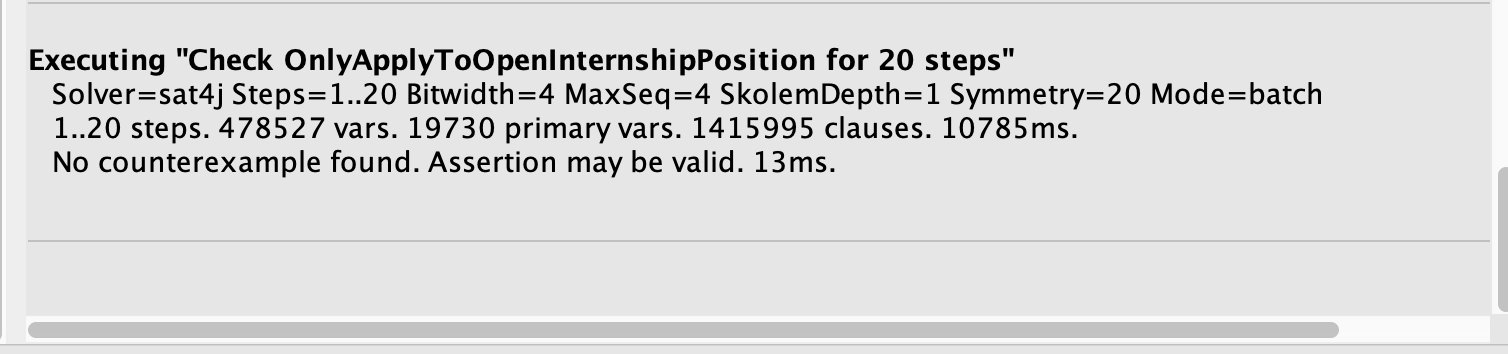
\includegraphics[width=0.5\textwidth]{RASD/Images/Alloy/checkOnlyApplyToOpenInternshipPosition.png}
    \label{fig:checkOnlyApplyToOpenInternshipPosition}
\end{figure}
\begin{figure}[h!]
    \centering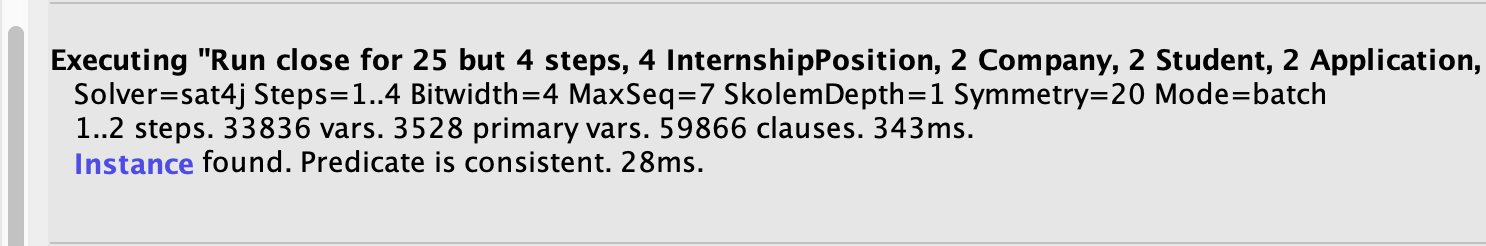
\includegraphics[width=0.5\textwidth]{RASD/Images/Alloy/predclose.png}
    \label{fig:predclose}
\end{figure}
\begin{figure}[h!]
    \centering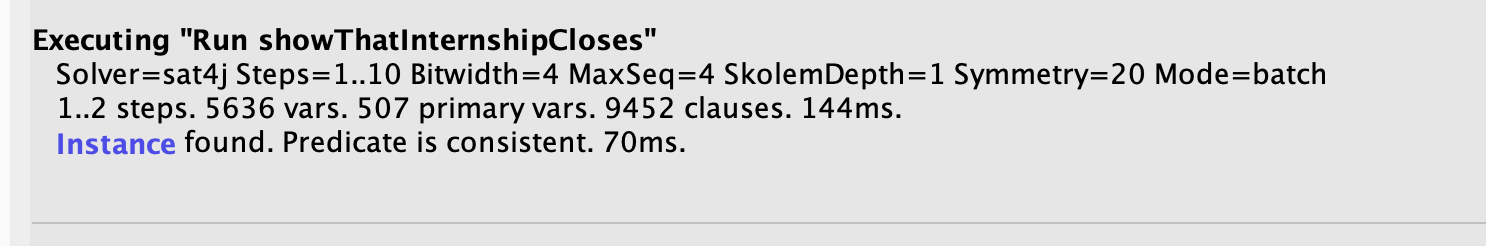
\includegraphics[width=0.5\textwidth]{RASD/Images/Alloy/predshowThatInternshipCloses.png}
    \label{fig:predshowThatInternshipCloses}
\end{figure}
\newpage
\begin{verbatim}
--------------------------------------------------------------------------------
Applications
--------------------------------------------------------------------------------

// All applications are done to open positions
fact ApplicationsOnlyForOpenPositions {
    all a: Application | a.internshipPosition.status = Open
}

// All applications are pending at the beginning
fact DefaultPendingApplication {
    all a: Application | a.status = Pending
}

// If an application is pending or to be assessed, it will eventually be either rejected or confirmed or refused
fact EventualStatusOfPendingApplication {
    all a: Application | 
        always ( a.status = Pending or a.status = ToBeAssessed
                implies 
                    eventually a.status = Rejected or 
                    a.status = Confirmed or a.status = Refused )
}

// Pending applications are referred only to open internship positions
assert PendingApplicationReferToOpenPositions {
    all a: Application | 
        a.status = Pending implies a.internshipPosition.status = Open
}

// Applications which request further assessment are referred only to open internship positions
assert TobeAssessedApplicationReferToOpenPositions {
    all a: Application | 
        a.status = ToBeAssessed implies a.internshipPosition.status = Open
}
\end{verbatim}
The results of the instructions above:
\begin{figure}[h!]
    \centering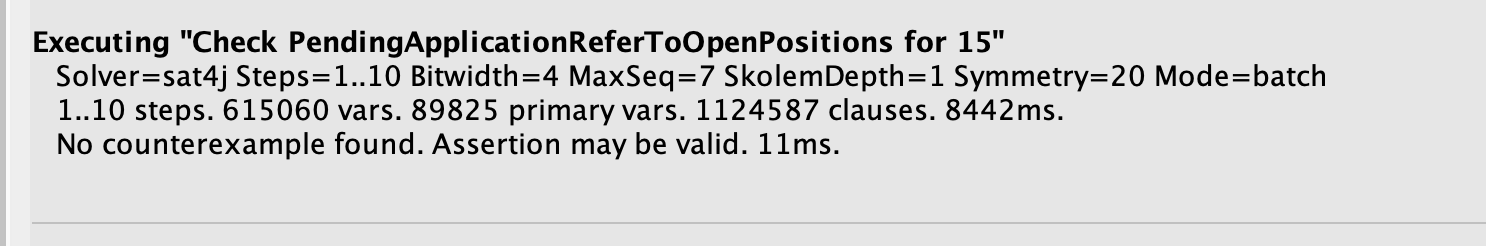
\includegraphics[width=0.5\textwidth]{RASD/Images/Alloy/checkPendingApplicationsReferToOpenPositions.png}
    \label{fig:checkPendingApplicationsReferToOpenPositions}
\end{figure}
\begin{figure}[h!]
    \centering\includegraphics[width=0.5\textwidth]{RASD/Images/Alloy/checkTobeAssessedApplicationReferToOpenPositions.png}
    \label{fig:TobeAssessedApplicationReferToOpenPositions}
\end{figure}
\newpage
\begin{verbatim}
--------------------------------------------------------------------------------
Internships
--------------------------------------------------------------------------------

// All internships are ongoing at the beginning
fact DefaultInternship {
    all i: Internship | i.status = Ongoing
}

// All internships refer to confirmed application 
fact AllInternshipReferToConfirmedApplication {
    all i: Internship | i.application.status = Confirmed
}

// If an internship is ongoing, it will eventually be finished
fact NotAlwaysOngoingInternship {
    all i: Internship | 
        always ( i.status = Ongoing
                implies 
                    eventually i.status = Finished )
}

// If an internship is nongoing it has been ongoing since the beginning
fact NowOpenPreviouslyOpenInternship {
    all i: Internship | 
        always ( i.status = Ongoing
                    implies 
                        historically i.status = Ongoing )
}

// If an internship is finished now it has been finished in an instant in the past
fact IfClosedDidCloseInternship {
all i: Internship |
    always (i.status = Finished
        implies 
            once finish[i])
}

pred finish[i: Internship] {
    i.status = Ongoing
    i.status' = Finished
}

run finish for 15 but 4 InternshipPosition, 2 Company, 2 Student, 2 Application, 
6 Internship, 2 University, 4 steps
\end{verbatim}

The results of the instructions above:
\begin{figure}[h!]
    \centering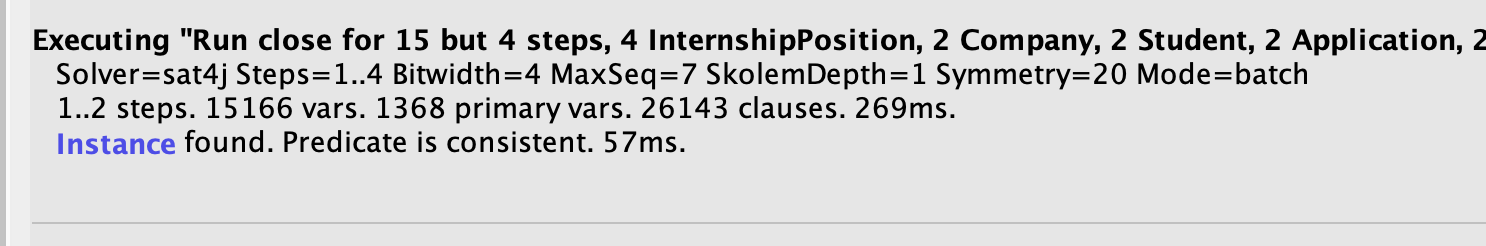
\includegraphics[width=0.5\textwidth]{RASD/Images/Alloy/predfinish.png}
    \label{fig:predfinish}
\end{figure}
\newpage
\begin{verbatim}
--------------------------------------------------------------------------------
Feedback 
--------------------------------------------------------------------------------

// All feedbacks given by student are given after an internship is finished
assert FeedbackStudentGivenOnFinishedInternship {
    all f: FeedbackByStudent | f.internship.status = Finished
}

// All feedbacks given by companies are given after an internship is finished
assert FeedbackCompanyGivenOnFinishedInternship {
    all f: FeedbackByCompany | f.internship.status = Finished
}

// A student can only give feedback for an internship he has taken
fact StudentFeedbackOnlyTheirInternship {
    all f: FeedbackByStudent | 
        f.giver in f.internship.application.student
}

// A company can only give feedback for an internship he has offered
fact CompanyFeedbackOnlyTheirInternship {
    all f: FeedbackByCompany | 
        f.giver in f.internship.application.company
}

check FeedbackCompanyGivenOnFinishedInternship for 10

\end{verbatim}

The results of the instructions above:

\begin{figure}[h!]
    \centering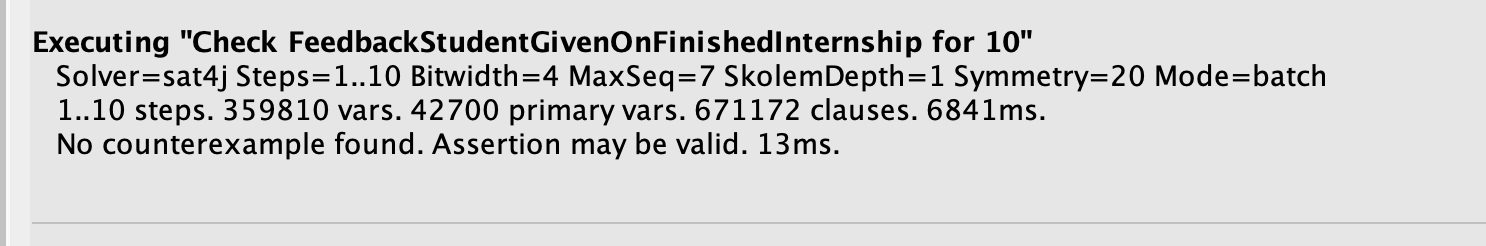
\includegraphics[width=0.5\textwidth]{RASD/Images/Alloy/checkFeedbackStudentGivenOnFinishedInternship.png}
    \label{fig:checkFeedbackStudentGivenOnFinishedInternship}
\end{figure}
\newpage
\begin{verbatim}
   
--------------------------------------------------------------------------------
Complaints 
--------------------------------------------------------------------------------

// All complaints given by student are given during an internship 
fact ComplaintByStudentDuringInternship {
    all f: ComplaintByStudent | f.internship.status = Ongoing
}

// All complaints given by companies are given during an internship 
fact ComplaintByCompanyDuringInternship {
    all f: ComplaintByCompany | f.internship.status = Ongoing
}

// A student can only complain about an internship he is taking
fact StudentComplainsOnlyTheirInternship {
    all f: ComplaintByStudent | 
        f.giver in f.internship.application.student
}

// A company can only complain about an internship it is offering
fact CompanyComplainsOnlyTheirInternship {
    all f: ComplaintByCompany | 
        f.giver in f.internship.application.company
}
\end{verbatim}
\begin{verbatim}
--------------------------------------------------------------------------------
Universities 
--------------------------------------------------------------------------------

// University sees the applications of its own students 
fact UniversityMonitorsItsStudentsInternship {
    all u: University, i: Internship | 
        i in u.internship implies i.application.student.university = u
}

\end{verbatim}
\begin{figure}[h!]
    \centering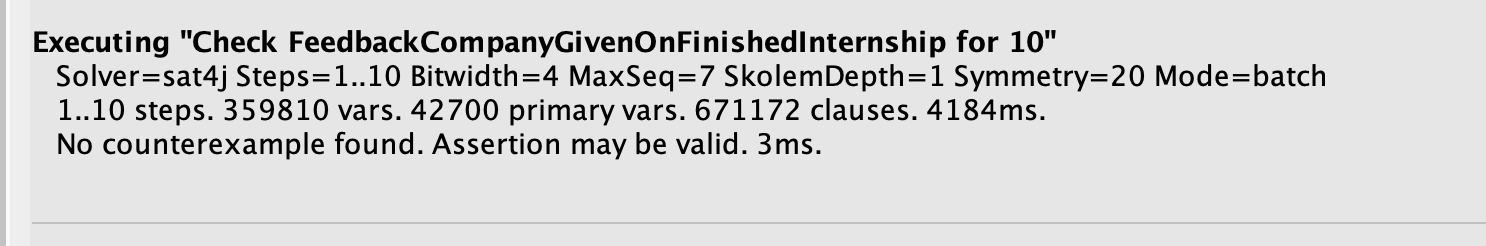
\includegraphics[width=0.5\textwidth]{RASD/Images/Alloy/checkFeedbackCompanyGivenOnFinishedInternship.png}
    \label{fig:checkFeedbackCompanyGivenOnFinishedInternship}
\end{figure}



%------------------------------------------------------------------------------------------------------------------------------------------------
\clearpage
{\color{Blue}{\section{Effort Spent}}}
\label{sect:effort}
%Provide here information about how much effort each group member spent in working at this document. We would appreciate details here.




\section*{Project Working Hours}

\begin{table}[ht!]
\centering
\adjustbox{max width=\textwidth}{
\begin{tabular}{|p{6cm}|p{2.5cm}|p{2.5cm}|p{2.5cm}|}
\hline
\textbf{Project Section} & \textbf{Gribaldo (hours)} & \textbf{Rosa (hours)} & \textbf{Total Hours} \\
\hline
\textbf{ 1) Introduction}                   & 3.5   & 2:30   & 0   \\
\textbf{ 2) Overall Description}            & 5     & 8:30   & 0   \\
\textbf{ 3) Specific Requirements}          & 0     & 2:20   & 0   \\
\textbf{ 4) Formal Analysis using Alloy}    & 0     & 0      & 0   \\
\hline
\textbf{Total Hours}                        & 0     & 0     & 0   \\
\hline
\end{tabular}
}
\caption{Working Hours per Project Section}
\label{tab:working_hours}
\end{table}

\vspace*{\fill}






%------------------------------------------------------------------------------------------------------------------------------------------------
\clearpage
\addcontentsline{toc}{section}{References}
\bibliographystyle{plain}
\bibliography{main}
%------------------------------------------------------------------------------------------------------------------------------------------------




\end{document}
